
% This is a simple template for a LaTeX document using the "article" class.
% See "book", "report", "letter" for other types of document.

\documentclass[10pt]{article} % use larger type; default would be 10pt

\usepackage[T1]{fontenc}
% \usepackage[french]{babel}
\usepackage[utf8]{inputenc} % set input encoding (not needed with XeLaTeX)
\usepackage{kpfonts}
\usepackage{hyperref}
\usepackage{epigraph}
\usepackage[french]{babel}
\usepackage{listings}
\usepackage{theorem}

\newtheorem{definition}{Définition}[subsection]

%%% Examples of Article customizations
% These packages are optional, depending whether you want the features they provide.
% See the LaTeX Companion or other references for full information.

%%% PAGE DIMENSIONS
\usepackage{geometry} % to change the page dimensions
\geometry{a4paper} % or letterpaper (US) or a5paper or....
% THE MARGINS FOR DSA is 1.5cm
\geometry{margin=1in}
% \geometry{margin=1.5cm} % for example, change the margins to 2 inches all round
% \geometry{landscape} % set up the page for landscape
%   read geometry.pdf for detailed page layout information


% \usepackage[parfill]{parskip} % Activate to begin paragraphs with an empty line rather than an indent

%%% PACKAGES
\usepackage{booktabs} % for much better looking tables
\usepackage{array} % for better arrays (eg matrices) in maths
\usepackage{paralist} % very flexible & customisable lists (eg. enumerate/itemize, etc.)
\usepackage{verbatim} % adds environment for commenting out blocks of text & for better verbatim
% \usepackage{subfig} % make it possible to include more than one captioned figure/table in a single float
% These packages are all incorporated in the memoir class to one degree or another...

%%% HEADERS & FOOTERS
\usepackage{fancyhdr} % This should be set AFTER setting up the page geometry
% \pagestyle{fancy} % options: empty , plain , fancy

\usepackage{graphicx} % support the \includegraphics command and options
\usepackage{subcaption}
\usepackage{caption}

\usepackage{dingbat} % For the pointy hands
\usepackage{pifont}
% \usepackage{xcolor} % For pretty colors
\usepackage[table]{xcolor}
\usepackage{tikz} % for nice pictures
\usepackage{blindtext}
\usepackage{wrapfig}
\usepackage{gensymb}
% \usepackage{table}

% COLORs
\definecolor{mygold}{RGB}{182, 153, 45}
\definecolor{mygreen}{RGB}{62, 171, 0}
\definecolor{dullgreen}{RGB}{165, 181, 45}
\definecolor{mypurp}{RGB}{84, 45, 181}


% \renewcommand{\headrule}{\color{gray}}
\renewcommand{\headrule}{\hbox to\headwidth{%
  \color{gray}\leaders\hrule height \headrulewidth\hfill}}

\renewcommand{\footrulewidth}{1pt}
% \renewcommand{\footrule}{\hbox to\headwirth{
%     \color{gray}\leaders\hrule height \footrulewidth\hfill}}

\renewcommand{\footrule}{{\color{gray}\vskip-\footruleskip\vskip-\footrulewidth \hrule width\headwidth height\footrulewidth\vskip\footruleskip}}

\fancyhf{}
% \rhead{\textcolor{gray}{Séance TP 1}}
\chead{\color{gray} Câbles Sous-marin}
% \lhead{Optimisation du GCC}
% \lfoot{\color{gray}\textcopyright 2022 Evan Voyles}
% \rfoot{\color{gray} Page \thepage\ sur 3}
\cfoot{\color{gray}Spécialité MAIN-3}
% \footskip = 0pt
% \voffset = 10pt
% \headsep = 0pt
% \cfoot{\thepage\ of \pageref{LastPage}}

% \renewcommand{\headrulewidth}{0pt} % customise the layout...
% \lhead{}\chead{}\rhead{}
% \lfoot{}\cfoot{\thepage}\rfoot{}

% \usepackage{}
\usepackage[absolute,overlay]{textpos} % Add text in any arbitrary position
% \usepackage{biblatex}

%%% SECTION TITLE APPEARANCE
\usepackage{sectsty}
\allsectionsfont{\sffamily\mdseries\upshape} % (See the fntguide.pdf for font help)
% (This matches ConTeXt defaults)

%%% ToC (table of contents) APPEARANCE
\usepackage[nottoc,notlof,notlot]{tocbibind} % Put the bibliography in the ToC
\usepackage[titles,subfigure]{tocloft} % Alter the style of the Table of Contents
\renewcommand{\cftsecfont}{\rmfamily\mdseries\upshape}
\renewcommand{\cftsecpagefont}{\rmfamily\mdseries\upshape} % No bold!

%%% END Article customizations

%%% The "real" document content comes below...

\newcommand{\asgold}[1]{\textcolor{mygold}{{\bf#1}}}
\newcommand{\asgrey}[1]{\textcolor{gray}{{\bf#1}}}
\newcommand{\asred}[1]{\textcolor{red}{{\bf#1}}}
\newcommand{\asor}[1]{\textcolor{orange}{{\bf#1}}}
\newcommand{\ascy}[1]{\textcolor{cyan}{{\bf#1}}}
\newcommand{\asgr}[1]{\textcolor{mygreen}{{\bf#1}}}
\newcommand{\aspurp}[1]{\textcolor{mypurp}{{\bf#1}}}

%%% LSTLISTINGS CONFIG:
\lstset{ %
  backgroundcolor=\color{white},   % choose the background color; you must add \usepackage{color} or \usepackage{xcolor}
  basicstyle=\footnotesize,        % the size of the fonts that are used for the code
  breakatwhitespace=false,         % sets if automatic breaks should only happen at whitespace
  breaklines=true,                 % sets automatic line breaking
  captionpos=b,                    % sets the caption-position to bottom
  commentstyle=\color{red}\textit,    % comment style
  deletekeywords={set, min, max, seq},            % if you want to delete keywords from the given language
  escapeinside={\%*}{*)},          % if you want to add LaTeX within your code
  extendedchars=true,              % lets you use non-ASCII characters; for 8-bits encodings only, does not work with UTF-8
  frame=tb,	                   	   % adds a frame around the code
  keepspaces=true,                 % keeps spaces in text, useful for keeping indentation of code (possibly needs columns=flexible)
  keywordstyle=\color{blue}\bfseries,       % keyword style
  language=R,                 % the language of the code (can be overrided per snippet)
  otherkeywords={*,...},           % if you want to add more keywords to the set
  numbers=left,                    % where to put the line-numbers; possible values are (none, left, right)
  numbersep=5pt,                   % how far the line-numbers are from the code
  numberstyle=\tiny\color{green}, % the style that is used for the line-numbers
  rulecolor=\color{black},         % if not set, the frame-color may be changed on line-breaks within not-black text (e.g. comments (green here))
  showspaces=false,                % show spaces everywhere adding particular underscores; it overrides 'showstringspaces'
  showstringspaces=false,          % underline spaces within strings only
  showtabs=false,                  % show tabs within strings adding particular underscores
  stepnumber=1,                    % the step between two line-numbers. If it's 1, each line will be numbered
  stringstyle=\color{purple}, % string literal style
  tabsize=2,	                   % sets default tabsize to 2 spaces
  title=\lstname,                  % show the filename of files included with \lstinputlisting; also try caption instead of title
  columns=fixed                    % Using fixed column width (for e.g. nice alignment)
}

\title{Simulation conditionnelle d'un processus gaussien}
\author{NEEL Pauline, PETROS Russom Samson, RAKOTOVAO Jonathan, VOYLES Evan}
\date{20 Mai 2022}


\begin{document}


\begin{titlepage}

\maketitle

\begin{figure}[h!]
    \centering
    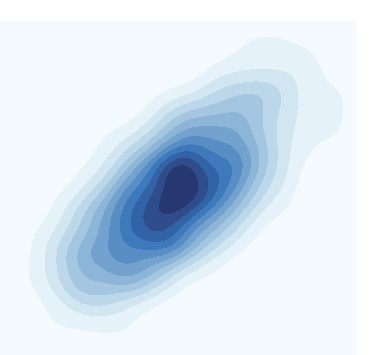
\includegraphics{media/plot.png}
\end{figure}

\vspace{3cm}

% \begin{figure}[h!]
%     \centering
%     
\includegraphics[width=0.25\linewidth]{media/1280px-Logo_Polytech_Sorbonne.png}
% \end{figure}

% \begin{abstract}
% Abstract.

% \end{abstract}

% \renewcommand {\epigraphflush} {center}

\epigraph{Any one who considers arithmetical methods of producing random digits is, of course, in a state of sin}
 {\textit{John von Neumann}}

\newpage

\end{titlepage}

\pagestyle{fancy}

\tableofcontents

\newpage

\section{Introduction}

L’objectif principal de ce projet est d’étudier et d’implémenter une procédure permettant de générer des simulations conditionnelles de processus gaussiens à l’aide de la méthode spectrale et du krigeage. Nous procéderons pour cela pas à pas.

La première étape sera d’abord d’appréhender ce qu’est un algorithme de simulation et de comprendre comment cela fonctionne. Nous commencerons donc ce projet par une question simple : comment générer des réalisations d’une variable aléatoire normale (cadre univarié). Pour y répondre, nous allons s’intéresser à la méthode d’acceptation-rejet ainsi qu’à la méthode de Box-Muller.

On se placera ensuite dans un cadre multivarié : nous utiliserons la décomposition de Cholesky de la matrice de variance-covariance afin de générer des réalisations d’un vecteur gaussien. Enfin, dans un cadre spatial, nous simulerons des processus gaussiens grâce à la méthode spectrale, puis conditionnerons les simulations obtenues à l’aide du krigeage. L’implémentation des différents algorithmes se fera sous R.

De plus, en utilisant Rshiny nous coderons une application web qui permettra à des utilisateurs de générer puis de visualiser des réalisations de variables aléatoires, vecteurs ou processus gaussiens.


\section{Simulation classique}
\subsection{Génération de variables aléatoires}


Un ordinateur n'est qu'un gros agencement complexe de circuits. Régnées par les lois physiques, les opérations provenant du mouvement des électrons
sont encodées par les fonctions booléennes. Les \textit{fonctions} - dans le sens mathématique - sont des objets purement déterministes. Autrement dit,
une fonction associe à une donnée d'entrée, une unique valeur dans l'espace d'arrivée.

Si on lui donne plusieurs fois la même valeur, par exemple $x_1$ et $x_2$
telles que $x_1 = x_2$, la définition d'une fonction implique que $f(x_1) = f(x_2)$. D'où vient l'énigme : Comment générer des variables aléatoires alors que nous
disposons seulement de méthodes déterministes?
% \setlength \epigraphwidth {\linewidth}

Nous ne pouvons pas à répondre à cette question plus éloquemment que le fait John von Neumann, l'un des meilleurs mathématiciens, pionniers, informaticiens de tous les temps; générer des variables aléatoires sur un ordinateur est tout simplement impossible.
Cependant, cela ne nous empêchera pas d'essayer quand même. Il s'agira de produire des variables dites pseudo-aléatoires.

\subsection{Loi uniforme}

On commence notre projet en étudiant la loi la plus simple parmi les lois usuelles - la loi uniforme. Tout d'abord, parce qu'elle est simple, mais la loi uniforme va également nous permettre de construire des algorithmes plus complexes, notamment la méthode de la transformée inverse ou la méthode de rejet. Ainsi, cela nous permettra de simuler différentes lois, comme la loi normale, la loi exponentielle, etc.

Il s'agira principalement d'échantillonner une variable $X\sim \mathcal{U}(0, 1)$ puis ensuite d'effectuer des manipulations mathématiques pour produire une variable suivant une autre loi ciblée.

Alors sans plus tarder, on formalise nos objectifs. Le principe est le suivant: nous allons générer une suite $(x_n$) à partir d'une graine $x_0$ et une fonction $f : \mathbb{R} \longrightarrow \mathbb{R}$ telles que
$$
\left\{
    \begin{array}{ll}
        x_{0} \in \mathbb{R} \\
        x_{n} = f(x_{n - 1})  \quad \forall n \in \mathbb{N} \\
    \end{array}
\right.
$$

On souhaite trouver une fonction qui vérifie certaines qualités désirées. Par exemple, on veut que notre fonction ait une période suffisamment longue. En effet, nous savons qu'elle sera périodique, il est donc importante que sa période soit très grande pour pas qu'un schéma soit visible.

On souhaite également qu'elle
produise des valeurs uniformément réparties sur un intervalle. Etudions la fonction $x \mapsto (x + 1) \mathbin{\%} 2$, où \% est l'opération de modulos et on fixe une graine $x_0 = 1$.
\begin{align*}
    f(x_0) &= (1 + 1) \mathbin{\%} 2 = 2 \mathbin{\%} 2 = 0 \\
    f(x_1) &= (0 + 1) \mathbin{\%} 2 = 1 \mathbin{\%} 2 = 1 \\
    f(x_2) &= (1 + 1) = 0
\end{align*}
Cette fonction produit alors la suite
\begin{equation*}
    \{1, 0, 1, 0, 1, 0, 1, 0, ...\}
\end{equation*}
dont la période est 2 et évidemment dont les valeurs ne sont pas aussi variées qu'on le souhaite. Nous verrons plus précisement ce que
``suffisamment variés'' veut dire. Pour l'instant, on se contente de dire que cette suite-là n'atteint pas nos attentes.

Heureusement pour nous, il existe de nombreuses fonctions
qui remplissent nos critères recherchés, ce sont des fonctions pseudo-aléatoires, elles sont déterminées mais leurs comportements s'approchent de l'aléatoire.

\subsubsection{Générateur congruentiel linéaire}

La méthode la plus directe à implémenter pour générer une telle suite est un \textit{générateur congruentiel linéaire}. Congruentiel parce qu'il s'agit d'une opération modulo et
linéaire vu qu'il y a une transformation affine. Dans le cas général, on considère les fonctions de la forme:
$$
    f(x; a, c, m) = (ax + c) \bmod m.
$$

D'ailleurs, la fonction étudiée dans la section précédente est un générateur congruentiel linéaire dont les paramètres sont $a = 1$, $c = 1$, et $m = 2$. Ne vous inquiétez pas, il existe un large panel de
générateurs congruentiels linéaires (LCG). Les choix des paramètres utilisés par les logiciels connus sont détaillés sur une page Wikipédia et leurs propriétés sont déjà
bien étudiées. Vu que l'objectif de notre projet est d'approfondir la connaissance autour des méthodes générant des variables (pseudo) aléatoires, on a décidé d'implémenter notre propre LCG hybride.
Pour $m$, on choisit $2^{31} - 1$, un nombre de Mersenne qui est très connu. Pour $a$, on s'amuse en choisissant $12345678$. Finalement, on affecte à l'incrémenteur $c$ la valeur 1.
$$
    f_{sousmarin}(x) = (12345678x + 1) \bmod (2^{31} - 1)
$$


\subsubsection{Implémentation en R}
Dans ce projet, nous faisons le choix d'implémenter notre propre version de runif afin de comprendre en profondeur la notion d'aléatoire. En effet, toutes les autres lois que nous allons pouvoir simuler, seront constuites à partir de runif. Il était donc important pour nous de faire cette étape. Afin d'implémenter une version de notre fonction en language de programmation R, on doit s'éloigner un peu de la pureté de la théorie et se salir les mains dans le code ! C'est-à-dire que l'on ne va pas garder une valeur $x_0$
pour toute l'éternité; on aura une variable globale déterminant l'état du générateur qui serait mise à jour quand on veut générer une suite de valeurs.

% \lstset{language=R, caption=somecaption, keywords={smooth}}

\begin{lstlisting}[language =R]

    # Initialiser la graine (une variable globale) a 0
    g_SEED_SOUSMARIN <- 0

    # similaire a la fonction de R set.seed, mettre a jour
    # la valeur de g_SEED_SOUSMARIN
    set_seed <- function(seed) {
        assign("g_SEED_SOUSMARIN", seed, envir = .GlobalEnv)
    }

    # La fonction LCG pure qu'on a definie en partie 3
    f_sousmarin <- function(x) {
        (12345678 * x + 1) %% (2^31 - 1)
    }

    # Generer une suite des variables de taille n en mettant a jour l'etat
    # de la graine a chaque pas.
    gen_suite <- function(n) {

        suite <- vector("numeric", n) # allouer un vecteur de taille n

        for (i in seq_len(n)) {
            x_i <- f_sousmarin(g_SEED_SOUSMARIN)
            suite[[i]] <- x_i
            set_seed(x_i)
        }

        suite
    }
\end{lstlisting}

On a donc implémenté notre propre LCG, \texttt{f\_sousmarin}. Pour renvoyer une valeur dans l'intervalle ]0, 1[ afin de simuler $X \sim \mathcal{U}(0, 1)$, on remarque que
la division modulo $m$ renvoie une valeur entre ]0, $m - 1$[. Pour le normaliser, on divise par le facteur $m - 1 \equiv 2^{31} - 2$.

\begin{lstlisting}[language=R]

    r_std_unif <- function(n) {

        suite <- vector("numeric", n)

        for (i in seq_len(n)) {
            x_i <- f_sousmarin(g_SEED_SOUSMARIN)
            suite[[i]] <- x_i / (2^31 - 2)
            set_seed(x_i)
        }

        suite
    }

\end{lstlisting}

Si on considère le cas général où l'on souhaiterait générer des variables uniformément réparties dans l'intervalle ]$a$, $b$[, on commence tout d'abord
par échantillonner $X \sim \mathcal{U}(0, 1)$. Ensuite, on multiplie $X$ par l'écart entre $a$ et $b$, ($b - a$), pour produire une variable $X_{b - a} \in$ ]$0$, $b - a$[. Finalement,
on décale $X_{b - a}$ en additionnant $a$ pour finir avec la variable aléatoire uniformément répartie dans l'intervalle ]$0 + a, b - a + a$[ $\equiv $ ]$a, b$[. Après cette transformation affine appliquée à
$X$, nous avons $X_{a,b} \sim \mathcal{U}(a, b)$.

On imite le comportement et la signature de la fonction dans R de base \texttt{runif} avec l'implémentation suivante

\begin{lstlisting}[language=R]

    r_unif <- function(n, min = 0, max = 1) {

        spread <- max - min
        suite  <- vector("numeric", n)

        for (i in seq_len(n)) {
            x_i <- f_sousmarin(g_SEED_SOUSMARIN)
            suite[[i]] <- (x_i * spread) / (2^31 - 2) + min
            set_seed(x_i)
        }

        suite
    }

\end{lstlisting}


\subsubsection{Vérification pour la loi uniforme}

Comment vérifier que notre LCG produit des valeurs qui sont véritablement réparties uniformément ? Quand il s'agit de produire
des milliards d'observations, on ne peut pas facilement vérifier à la main si notre fonction n'a pas de structure évidente (sauf la période qui est mathématiquement inévitable).
Pourtant, on peut commencer par une exploration visuelle.

Pour ce faire, on utilise la fonction \texttt{r\_std\_unif} définie au-dessus pour générer 1E6 valeurs aléatoires qui sont supposées être uniformément
réparties sur l'intervalle ]$0, 1$[.

\begin{figure}[h!]
    \centering
    % Created by tikzDevice version 0.12.3.1 on 2022-03-15 02:59:11
% !TEX encoding = UTF-8 Unicode
\begin{tikzpicture}[x=1pt,y=1pt]
\definecolor{fillColor}{RGB}{255,255,255}
\path[use as bounding box,fill=fillColor,fill opacity=0.00] (0,0) rectangle (361.35,216.81);
\begin{scope}
\path[clip] (  0.00,  0.00) rectangle (361.35,216.81);
\definecolor{drawColor}{RGB}{255,255,255}
\definecolor{fillColor}{RGB}{255,255,255}

\path[draw=drawColor,line width= 0.6pt,line join=round,line cap=round,fill=fillColor] (  0.00,  0.00) rectangle (361.35,216.81);
\end{scope}
\begin{scope}
\path[clip] ( 44.91, 30.69) rectangle (355.85,211.31);
\definecolor{fillColor}{gray}{0.92}

\path[fill=fillColor] ( 44.91, 30.69) rectangle (355.85,211.31);
\definecolor{drawColor}{RGB}{255,255,255}

\path[draw=drawColor,line width= 0.3pt,line join=round] ( 44.91, 71.16) --
	(355.85, 71.16);

\path[draw=drawColor,line width= 0.3pt,line join=round] ( 44.91,135.70) --
	(355.85,135.70);

\path[draw=drawColor,line width= 0.3pt,line join=round] ( 44.91,200.23) --
	(355.85,200.23);

\path[draw=drawColor,line width= 0.3pt,line join=round] ( 94.38, 30.69) --
	( 94.38,211.31);

\path[draw=drawColor,line width= 0.3pt,line join=round] (165.05, 30.69) --
	(165.05,211.31);

\path[draw=drawColor,line width= 0.3pt,line join=round] (235.71, 30.69) --
	(235.71,211.31);

\path[draw=drawColor,line width= 0.3pt,line join=round] (306.38, 30.69) --
	(306.38,211.31);

\path[draw=drawColor,line width= 0.6pt,line join=round] ( 44.91, 38.90) --
	(355.85, 38.90);

\path[draw=drawColor,line width= 0.6pt,line join=round] ( 44.91,103.43) --
	(355.85,103.43);

\path[draw=drawColor,line width= 0.6pt,line join=round] ( 44.91,167.97) --
	(355.85,167.97);

\path[draw=drawColor,line width= 0.6pt,line join=round] ( 59.04, 30.69) --
	( 59.04,211.31);

\path[draw=drawColor,line width= 0.6pt,line join=round] (129.71, 30.69) --
	(129.71,211.31);

\path[draw=drawColor,line width= 0.6pt,line join=round] (200.38, 30.69) --
	(200.38,211.31);

\path[draw=drawColor,line width= 0.6pt,line join=round] (271.05, 30.69) --
	(271.05,211.31);

\path[draw=drawColor,line width= 0.6pt,line join=round] (341.72, 30.69) --
	(341.72,211.31);
\definecolor{drawColor}{RGB}{0,0,0}
\definecolor{fillColor}{RGB}{16,118,212}

\path[draw=drawColor,line width= 0.6pt,line cap=rect,fill=fillColor] ( 59.04, 38.90) rectangle ( 62.58,201.64);

\path[draw=drawColor,line width= 0.6pt,line cap=rect,fill=fillColor] ( 62.58, 38.90) rectangle ( 66.11,199.58);

\path[draw=drawColor,line width= 0.6pt,line cap=rect,fill=fillColor] ( 66.11, 38.90) rectangle ( 69.64,200.31);

\path[draw=drawColor,line width= 0.6pt,line cap=rect,fill=fillColor] ( 69.64, 38.90) rectangle ( 73.18,200.42);

\path[draw=drawColor,line width= 0.6pt,line cap=rect,fill=fillColor] ( 73.18, 38.90) rectangle ( 76.71,200.22);

\path[draw=drawColor,line width= 0.6pt,line cap=rect,fill=fillColor] ( 76.71, 38.90) rectangle ( 80.24,202.65);

\path[draw=drawColor,line width= 0.6pt,line cap=rect,fill=fillColor] ( 80.24, 38.90) rectangle ( 83.78,196.18);

\path[draw=drawColor,line width= 0.6pt,line cap=rect,fill=fillColor] ( 83.78, 38.90) rectangle ( 87.31,201.56);

\path[draw=drawColor,line width= 0.6pt,line cap=rect,fill=fillColor] ( 87.31, 38.90) rectangle ( 90.84,198.76);

\path[draw=drawColor,line width= 0.6pt,line cap=rect,fill=fillColor] ( 90.84, 38.90) rectangle ( 94.38,197.69);

\path[draw=drawColor,line width= 0.6pt,line cap=rect,fill=fillColor] ( 94.38, 38.90) rectangle ( 97.91,200.16);

\path[draw=drawColor,line width= 0.6pt,line cap=rect,fill=fillColor] ( 97.91, 38.90) rectangle (101.44,199.52);

\path[draw=drawColor,line width= 0.6pt,line cap=rect,fill=fillColor] (101.44, 38.90) rectangle (104.98,202.58);

\path[draw=drawColor,line width= 0.6pt,line cap=rect,fill=fillColor] (104.98, 38.90) rectangle (108.51,199.11);

\path[draw=drawColor,line width= 0.6pt,line cap=rect,fill=fillColor] (108.51, 38.90) rectangle (112.04,200.25);

\path[draw=drawColor,line width= 0.6pt,line cap=rect,fill=fillColor] (112.04, 38.90) rectangle (115.58,201.56);

\path[draw=drawColor,line width= 0.6pt,line cap=rect,fill=fillColor] (115.58, 38.90) rectangle (119.11,200.07);

\path[draw=drawColor,line width= 0.6pt,line cap=rect,fill=fillColor] (119.11, 38.90) rectangle (122.64,200.07);

\path[draw=drawColor,line width= 0.6pt,line cap=rect,fill=fillColor] (122.64, 38.90) rectangle (126.18,198.81);

\path[draw=drawColor,line width= 0.6pt,line cap=rect,fill=fillColor] (126.18, 38.90) rectangle (129.71,202.02);

\path[draw=drawColor,line width= 0.6pt,line cap=rect,fill=fillColor] (129.71, 38.90) rectangle (133.24,197.73);

\path[draw=drawColor,line width= 0.6pt,line cap=rect,fill=fillColor] (133.24, 38.90) rectangle (136.78,201.95);

\path[draw=drawColor,line width= 0.6pt,line cap=rect,fill=fillColor] (136.78, 38.90) rectangle (140.31,199.94);

\path[draw=drawColor,line width= 0.6pt,line cap=rect,fill=fillColor] (140.31, 38.90) rectangle (143.84,197.50);

\path[draw=drawColor,line width= 0.6pt,line cap=rect,fill=fillColor] (143.84, 38.90) rectangle (147.38,200.54);

\path[draw=drawColor,line width= 0.6pt,line cap=rect,fill=fillColor] (147.38, 38.90) rectangle (150.91,201.90);

\path[draw=drawColor,line width= 0.6pt,line cap=rect,fill=fillColor] (150.91, 38.90) rectangle (154.45,200.02);

\path[draw=drawColor,line width= 0.6pt,line cap=rect,fill=fillColor] (154.45, 38.90) rectangle (157.98,200.72);

\path[draw=drawColor,line width= 0.6pt,line cap=rect,fill=fillColor] (157.98, 38.90) rectangle (161.51,199.56);

\path[draw=drawColor,line width= 0.6pt,line cap=rect,fill=fillColor] (161.51, 38.90) rectangle (165.05,201.76);

\path[draw=drawColor,line width= 0.6pt,line cap=rect,fill=fillColor] (165.05, 38.90) rectangle (168.58,199.36);

\path[draw=drawColor,line width= 0.6pt,line cap=rect,fill=fillColor] (168.58, 38.90) rectangle (172.11,201.63);

\path[draw=drawColor,line width= 0.6pt,line cap=rect,fill=fillColor] (172.11, 38.90) rectangle (175.65,203.10);

\path[draw=drawColor,line width= 0.6pt,line cap=rect,fill=fillColor] (175.65, 38.90) rectangle (179.18,199.76);

\path[draw=drawColor,line width= 0.6pt,line cap=rect,fill=fillColor] (179.18, 38.90) rectangle (182.71,200.47);

\path[draw=drawColor,line width= 0.6pt,line cap=rect,fill=fillColor] (182.71, 38.90) rectangle (186.25,200.09);

\path[draw=drawColor,line width= 0.6pt,line cap=rect,fill=fillColor] (186.25, 38.90) rectangle (189.78,197.78);

\path[draw=drawColor,line width= 0.6pt,line cap=rect,fill=fillColor] (189.78, 38.90) rectangle (193.31,198.20);

\path[draw=drawColor,line width= 0.6pt,line cap=rect,fill=fillColor] (193.31, 38.90) rectangle (196.85,200.72);

\path[draw=drawColor,line width= 0.6pt,line cap=rect,fill=fillColor] (196.85, 38.90) rectangle (200.38,196.53);

\path[draw=drawColor,line width= 0.6pt,line cap=rect,fill=fillColor] (200.38, 38.90) rectangle (203.91,199.83);

\path[draw=drawColor,line width= 0.6pt,line cap=rect,fill=fillColor] (203.91, 38.90) rectangle (207.45,196.34);

\path[draw=drawColor,line width= 0.6pt,line cap=rect,fill=fillColor] (207.45, 38.90) rectangle (210.98,198.52);

\path[draw=drawColor,line width= 0.6pt,line cap=rect,fill=fillColor] (210.98, 38.90) rectangle (214.51,202.13);

\path[draw=drawColor,line width= 0.6pt,line cap=rect,fill=fillColor] (214.51, 38.90) rectangle (218.05,199.05);

\path[draw=drawColor,line width= 0.6pt,line cap=rect,fill=fillColor] (218.05, 38.90) rectangle (221.58,198.47);

\path[draw=drawColor,line width= 0.6pt,line cap=rect,fill=fillColor] (221.58, 38.90) rectangle (225.11,201.41);

\path[draw=drawColor,line width= 0.6pt,line cap=rect,fill=fillColor] (225.11, 38.90) rectangle (228.65,200.03);

\path[draw=drawColor,line width= 0.6pt,line cap=rect,fill=fillColor] (228.65, 38.90) rectangle (232.18,197.60);

\path[draw=drawColor,line width= 0.6pt,line cap=rect,fill=fillColor] (232.18, 38.90) rectangle (235.71,198.92);

\path[draw=drawColor,line width= 0.6pt,line cap=rect,fill=fillColor] (235.71, 38.90) rectangle (239.25,201.38);

\path[draw=drawColor,line width= 0.6pt,line cap=rect,fill=fillColor] (239.25, 38.90) rectangle (242.78,202.66);

\path[draw=drawColor,line width= 0.6pt,line cap=rect,fill=fillColor] (242.78, 38.90) rectangle (246.31,201.89);

\path[draw=drawColor,line width= 0.6pt,line cap=rect,fill=fillColor] (246.31, 38.90) rectangle (249.85,201.23);

\path[draw=drawColor,line width= 0.6pt,line cap=rect,fill=fillColor] (249.85, 38.90) rectangle (253.38,201.76);

\path[draw=drawColor,line width= 0.6pt,line cap=rect,fill=fillColor] (253.38, 38.90) rectangle (256.91,200.63);

\path[draw=drawColor,line width= 0.6pt,line cap=rect,fill=fillColor] (256.91, 38.90) rectangle (260.45,201.53);

\path[draw=drawColor,line width= 0.6pt,line cap=rect,fill=fillColor] (260.45, 38.90) rectangle (263.98,198.80);

\path[draw=drawColor,line width= 0.6pt,line cap=rect,fill=fillColor] (263.98, 38.90) rectangle (267.51,200.78);

\path[draw=drawColor,line width= 0.6pt,line cap=rect,fill=fillColor] (267.51, 38.90) rectangle (271.05,199.24);

\path[draw=drawColor,line width= 0.6pt,line cap=rect,fill=fillColor] (271.05, 38.90) rectangle (274.58,202.75);

\path[draw=drawColor,line width= 0.6pt,line cap=rect,fill=fillColor] (274.58, 38.90) rectangle (278.11,199.77);

\path[draw=drawColor,line width= 0.6pt,line cap=rect,fill=fillColor] (278.11, 38.90) rectangle (281.65,200.09);

\path[draw=drawColor,line width= 0.6pt,line cap=rect,fill=fillColor] (281.65, 38.90) rectangle (285.18,202.83);

\path[draw=drawColor,line width= 0.6pt,line cap=rect,fill=fillColor] (285.18, 38.90) rectangle (288.72,200.27);

\path[draw=drawColor,line width= 0.6pt,line cap=rect,fill=fillColor] (288.72, 38.90) rectangle (292.25,198.52);

\path[draw=drawColor,line width= 0.6pt,line cap=rect,fill=fillColor] (292.25, 38.90) rectangle (295.78,201.05);

\path[draw=drawColor,line width= 0.6pt,line cap=rect,fill=fillColor] (295.78, 38.90) rectangle (299.32,200.53);

\path[draw=drawColor,line width= 0.6pt,line cap=rect,fill=fillColor] (299.32, 38.90) rectangle (302.85,202.20);

\path[draw=drawColor,line width= 0.6pt,line cap=rect,fill=fillColor] (302.85, 38.90) rectangle (306.38,199.52);

\path[draw=drawColor,line width= 0.6pt,line cap=rect,fill=fillColor] (306.38, 38.90) rectangle (309.92,199.32);

\path[draw=drawColor,line width= 0.6pt,line cap=rect,fill=fillColor] (309.92, 38.90) rectangle (313.45,200.34);

\path[draw=drawColor,line width= 0.6pt,line cap=rect,fill=fillColor] (313.45, 38.90) rectangle (316.98,202.40);

\path[draw=drawColor,line width= 0.6pt,line cap=rect,fill=fillColor] (316.98, 38.90) rectangle (320.52,199.86);

\path[draw=drawColor,line width= 0.6pt,line cap=rect,fill=fillColor] (320.52, 38.90) rectangle (324.05,202.24);

\path[draw=drawColor,line width= 0.6pt,line cap=rect,fill=fillColor] (324.05, 38.90) rectangle (327.58,200.63);

\path[draw=drawColor,line width= 0.6pt,line cap=rect,fill=fillColor] (327.58, 38.90) rectangle (331.12,199.31);

\path[draw=drawColor,line width= 0.6pt,line cap=rect,fill=fillColor] (331.12, 38.90) rectangle (334.65,200.42);

\path[draw=drawColor,line width= 0.6pt,line cap=rect,fill=fillColor] (334.65, 38.90) rectangle (338.18,200.92);

\path[draw=drawColor,line width= 0.6pt,line cap=rect,fill=fillColor] (338.18, 38.90) rectangle (341.72,201.19);
\end{scope}
\begin{scope}
\path[clip] (  0.00,  0.00) rectangle (361.35,216.81);
\definecolor{drawColor}{gray}{0.30}

\node[text=drawColor,anchor=base east,inner sep=0pt, outer sep=0pt, scale=  0.88] at ( 39.96, 35.87) {0};

\node[text=drawColor,anchor=base east,inner sep=0pt, outer sep=0pt, scale=  0.88] at ( 39.96,100.40) {5000};

\node[text=drawColor,anchor=base east,inner sep=0pt, outer sep=0pt, scale=  0.88] at ( 39.96,164.94) {10000};
\end{scope}
\begin{scope}
\path[clip] (  0.00,  0.00) rectangle (361.35,216.81);
\definecolor{drawColor}{gray}{0.20}

\path[draw=drawColor,line width= 0.6pt,line join=round] ( 42.16, 38.90) --
	( 44.91, 38.90);

\path[draw=drawColor,line width= 0.6pt,line join=round] ( 42.16,103.43) --
	( 44.91,103.43);

\path[draw=drawColor,line width= 0.6pt,line join=round] ( 42.16,167.97) --
	( 44.91,167.97);
\end{scope}
\begin{scope}
\path[clip] (  0.00,  0.00) rectangle (361.35,216.81);
\definecolor{drawColor}{gray}{0.20}

\path[draw=drawColor,line width= 0.6pt,line join=round] ( 59.04, 27.94) --
	( 59.04, 30.69);

\path[draw=drawColor,line width= 0.6pt,line join=round] (129.71, 27.94) --
	(129.71, 30.69);

\path[draw=drawColor,line width= 0.6pt,line join=round] (200.38, 27.94) --
	(200.38, 30.69);

\path[draw=drawColor,line width= 0.6pt,line join=round] (271.05, 27.94) --
	(271.05, 30.69);

\path[draw=drawColor,line width= 0.6pt,line join=round] (341.72, 27.94) --
	(341.72, 30.69);
\end{scope}
\begin{scope}
\path[clip] (  0.00,  0.00) rectangle (361.35,216.81);
\definecolor{drawColor}{gray}{0.30}

\node[text=drawColor,anchor=base,inner sep=0pt, outer sep=0pt, scale=  0.88] at ( 59.04, 19.68) {0.00};

\node[text=drawColor,anchor=base,inner sep=0pt, outer sep=0pt, scale=  0.88] at (129.71, 19.68) {0.25};

\node[text=drawColor,anchor=base,inner sep=0pt, outer sep=0pt, scale=  0.88] at (200.38, 19.68) {0.50};

\node[text=drawColor,anchor=base,inner sep=0pt, outer sep=0pt, scale=  0.88] at (271.05, 19.68) {0.75};

\node[text=drawColor,anchor=base,inner sep=0pt, outer sep=0pt, scale=  0.88] at (341.72, 19.68) {1.00};
\end{scope}
\begin{scope}
\path[clip] (  0.00,  0.00) rectangle (361.35,216.81);
\definecolor{drawColor}{RGB}{0,0,0}

\node[text=drawColor,anchor=base,inner sep=0pt, outer sep=0pt, scale=  1.10] at (200.38,  7.64) {x};
\end{scope}
\begin{scope}
\path[clip] (  0.00,  0.00) rectangle (361.35,216.81);
\definecolor{drawColor}{RGB}{0,0,0}

\node[text=drawColor,rotate= 90.00,anchor=base,inner sep=0pt, outer sep=0pt, scale=  1.10] at ( 13.08,121.00) {count};
\end{scope}
\end{tikzpicture}


    \vspace{-1cm}
    \caption{Histogramme généré à partir d'un appel à \texttt{r\_std\_unif} avec $n = 1000000$. On initialise la graine de notre
    générateur avec un appel à \texttt{set\_seed(0)}.}

\end{figure}

On peut aussi facilement vérifier que les statistiques de notre échantillon correspondent bien à celles que l'on attend.

\begin{lstlisting}[language=R]
    library(sousmarin)

    set_seed(0)
    x <- r_std_unif(1E6)

    mu  <- mean(x) # 0.5000658
    sig <- std(x)  # 0.2877586
\end{lstlisting}

On réitère le simple fait qu'il n'y a \textbf{rien d'aléatoire} avec la génération de ces valeurs et que vous pouvez vérifier leur quantité en
téléchargeant notre package \textbf{ICI}\footnote{On mettra ici un lien du github (voire un lien de CRAN????) et des instructions pour télécharger notre package}.

On passe à l'analyse. Avec notre échantillon $x$ de taille 1E6, le moyen de l'échantillon $\bar x = 0.50006584$ et l'écart type de l'échantillon est $s = 0.2877586$.
Comme la moyenne d'une loi uniforme est $\frac{b - a}{2} = \frac{1 - 0}{2} = 0.5$, nous sommes ravis de voir que $\bar x = 0.50006584 \sim 0.5$. Parallèlement, l'écart type
d'une loi uniforme est $\frac{b - a}{\sqrt{12}} = \frac{1 - 0}{\sqrt{12}} = 0.2886751$, ce qui est proche de notre $s = 0.2877586$.


\subsubsection{Simulation de différentes lois}

Maintenant que nous avons compris la notion de "aléatoire" et de "pseudo-aléatoire", et que nous avons saisi comment fonctionne la fonction runif de R, nous allons pouvoir générer des variables aléatoires plus complexes. Dans la prochaine partie, nous allons implémenter la méthode de transformation inversée, pour simuler une loi exponentielle. Ensuite nous verrons la méthode d'acceptation-rejet pour simuler une loi normale, et Finalement la méthode de Box-Muller. Tous ces  algorithmes sont contruits à partir de runif, fonction de R qui distribue une variable aléatoire uniforme.

\subsection{Méthode de transformation inversée}

La méthode de transformation inversée consiste à échantillonner une variable aléatoire $X \sim \mathcal{U}(0, 1)$ et à utiliser l'expression analytique
de la fonction de répartition d'une loi cible. Comme la fonction de répartition $F(x$) est une fonction croissante définie sur $\mathbb{R}^n$ à valeurs dans
$[0, 1]$, si on peut trouver une expression fermée de son inverse $F^{-1} : [0, 1] \longrightarrow \mathbb{R}$, on applique la méthode de transformation inversée
afin de réaliser des simulations.

\subsubsection{Démonstration}
On pose :
\begin{align}
u = F(x) \Leftrightarrow x = F^{-1}(u)
\end{align}

Par définition, on a $F(x) = \mathbb{P}(X \leq  F^{-1}(u) )$.\
Il vient alors :
$F(F^{-1}(u)) = \mathbb{P}(X \leq F^{-1}(u) )$

Or, par définition de la réciproque :
$F(F^{-1}(u)) = u$ et comme F est strictement croissante : $\mathbb{P}(X \leq F^{-1}(u) )$.\
On en déduit que : $u = \mathbb{P}(F(X) \leq u )$ et on reconnaît la foncion de répartition de la loi uniforme.

Pour éclairer la méthode, on va étudier la fonction de répartition de la loi exponentielle. Pour rappel, une variable aléatoire suivant une loi exponentielle de paramètre
$\lambda$ a pour fonction de densité $f(x) = \lambda e^{-\lambda x}$ pour $x \geq 0$, $0$ sinon. On a choisi cette loi parce qu'elle est munie d'une fonction de répartition facilement calculable
et surtout dont l'inverse a une expression analytique. Calculons sa fonction de répartition:
\begin{align*}
    F(x) &= \int_{-\infty}^xf(t)dt \\
    & = \int_{-\infty}^0 0 dt + \int_0^x \lambda e^{-\lambda t} dt \\
    &= 0 + \left[-e^{-\lambda t}\right]_0^x \\
    &= 1 - e^{-\lambda x}
\end{align*}

Calculons maintenant son inverse, $F^{-1}$ :
\begin{align*}
    y &= 1 - e^{-\lambda (F^{-1}(y))} \\
    e^{\lambda (F^{-1}(y))} &= 1 - y \\
    -\lambda F^{-1}(y) &= \ln(1 - y) \\
    F^{-1}(y) &= \frac{-\ln(1 - y)}{\lambda}
\end{align*}

La loi exponentielle est l'une des quelques lois où l'on peut facilement trouver l'inverse de la fonction de répartition. Cela nous permet
d'échantilloner une variable aléatoire $X \sim \exp(\lambda)$ efficacement à partir d'une seule réalisation d'une loi uniforme. Il s'agit tout
simplement de tirer $U \sim \mathcal{U}(0, 1)$ et ensuite évaluer $X = F^{-1}(U)$.

L'implémentation en R ne prend qu'une seule ligne:

\begin{lstlisting}[language=R]
    rexp_inv <- function(n, lambda = 1) {
        # Generate n realizations of a uniform random variable n times
        (-1 / lambda) * log(runif(n, 0, 1))
    }
\end{lstlisting}

On peut facilement comparer la moyenne empirique avec la moyenne théorique. En effet, on sait que théoriquement, l'espérance de la loi
exponentielle de paramètre $\lambda$ est $\frac{1}{\lambda}$ Ainsi, on effectue la moyenne de $n = 1e4$ réalisations pour plusieurs
$\lambda$, et on compare ces résultats avec la théorie.

On obtient alors le graphique suivant qui montre que les moyennes empiriques calculées pour chaque lambda correspondent aux valeurs théoriques
de l'espérance.

\newpage

\begin{figure}[h!]
    \centering
    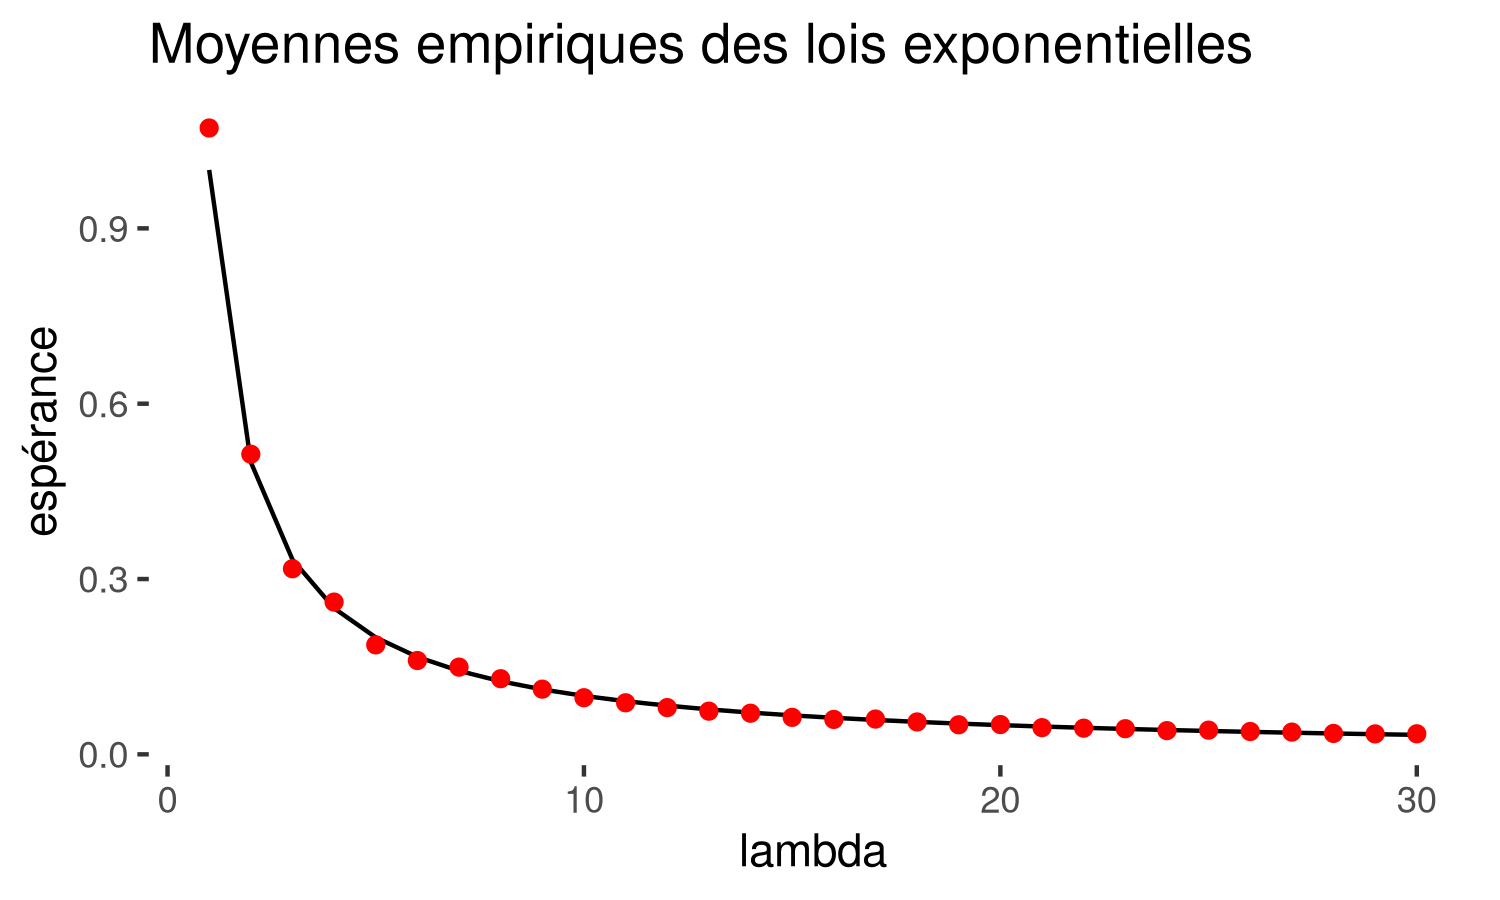
\includegraphics{media/moyenne_empiriques_exp.png}
    \caption{Comparaison moyennes empiriques avec espérance de plusiers lois exponentielles de paramètre $\lambda$.
    En rouge les moyennes empiriques. En noir les valeurs théoriques de l'espérance, $1/\lambda$.}
\end{figure}


\subsection{Méthode d'acceptation-rejet}

Comment faire lorsque l'on veut simuler une loi dont on ne peut pas calculer l'inverse de la fonction de répartition ? Une solution est d'utiliser la méthode d'acceptation-rejet.

\subsubsection{Démonstration}
Soit X une variable aléatoire de densité f et de fonction de répartition F.\
Supposons f nulle en dehors d'un intervalle [a,b].\
Soit M un majorant de f(x) : $\forall x \in [a,b] : f(x) \leq M$ \

On considère le graphe de la fonction $y = f(x)$ :

\begin{figure}[h!]
    \centering
    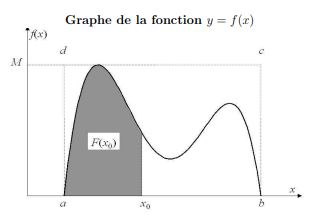
\includegraphics[width=0.6\textwidth]{media/Graphe_fonction.jpg}
\end{figure}

On a :
\begin{align}
\mathbb{P}(X \leq X_0) &= \mathbb{P}(X \leq  X_0 | A = (X, Y) ) \
&= \mathbb{P}(X \leq  X_0 | Y \leq f(x) )
\end{align}
ce qui donne, d'après la formule des probabilités conditionnelles :

\begin{align}
&= \frac{\mathbb{P}(X \leq  X_0, Y \leq f(x) )}{\mathbb{P}(Y \leq f(x))}
\end{align}
Or,

\begin{align}
\mathbb{P}(X \leq  X_0, Y \leq f(x) ) = \frac{\mathrm{surface\ de\ la\ zone\ hachurée}}{\mathrm{surface\ du\ rectangle\ (abcd)}} = \frac{F(X_0)}{M(b-a)}
\end{align}
et

\begin{align}
\mathbb{P}(X \leq  X_0, Y \leq f(x) ) = \frac{\mathrm{surface\ sous\ la\ courbe}}{\mathrm{surface\ du\ rectangle\ (abcd)}} = \frac{1}{M(b-a)}
\end{align}
On en déduit que :

\begin{align}
\mathbb{P}(X \leq X_0) = \frac{F(X_0)}{M(b-a)} x \frac{M(b-a)}{1}=F(X_0)
\end{align}
La variable X ainsi obtenue a bien une densité f et une fonction de
répartition F.

\subsubsection{Simulation}

Prenons un exemple simple pour mieux comprendre. Notons $f$ la fonction densité de loi que l'on souhaite simuler : $f(x) = 6x(1-x) $ sur le compact [0, 1] .

Le principe est simple : on va borner f par une fonction g que l'on sait simuler. Ici, on prendra la fonction constante $g(x) = 1.5 $. On simule des points uniformément répartis sous la courbe de $g(x)$. Supposons que l'on souhaite générer 10 simulations, on tire alors 10 réalisations de $X \sim \mathcal{U}(0, 1)$ : on aura les abscisses des points.

Ensuite, pour chaque abscisse, on tire $Y \sim \mathcal{U}(0, 1.5)$ ce qui représentera l'ordonnée de notre point. On aura alors tiré des points uniformément répartis dans le rectangle. Finalement, on garde seulement l'abscisse de ceux se trouvant en dessous de la fonction $f(x)$. Ainsi, l'ensemble de ces valeurs, les abscisses des points acceptés donc, seront bien distribuées selon la loi $f(x)$.

\begin{figure}[h!]
    \centering
    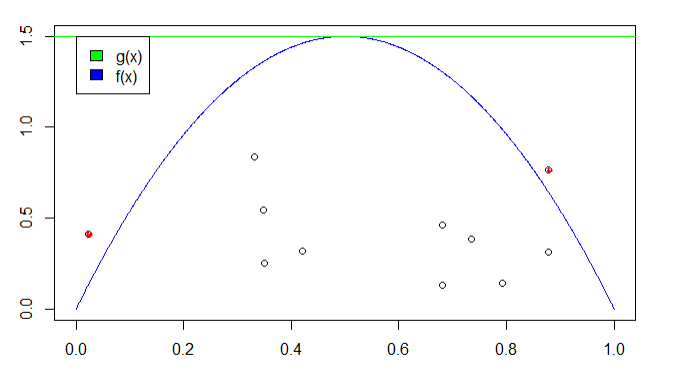
\includegraphics[width=.7\linewidth]{media/graph_acceptation_rejet.png}
    \caption{app shiny pour faire la simulation}
\end{figure}

Sur ce graphique, on voit que les points en rouge se situant au-dessus de $f(x)$ seront rejetés tandis que les points blancs se situant en-dessous de la courbe seront acceptés.

On peut facilement implémenter l'algorithme d'acceptation-rejet pour une loi quadratique suivant la densité $f(x) = 6x(1 - x)$ sur $[0, 1]$ sous R :
\begin{lstlisting}[language=R]
    rquad <- function(n) {

        ind <- function(x) { 0 <= x & x <= 1 } # x \in [0, 1]
        # Uniform density between (0, 1)
        f <- function(x) {
            6 * x * (1 - x) * ind(x)
        }

        g <- function(x) {
            1 * ind(x)
        }

        c <- 1.5
        out <- rep(0, n)

        for (i in seq_len(n)) {

            reject <- TRUE
            z <- 0

            while (reject) {

                y <- runif(1)
                u <- runif(1)

                reject <- u > (f(y) / (c * g(y)))
                z <- y
            }

            out[[i]] <- z
        }

        out
    }
\end{lstlisting}

On simule alors $n = 10,000$ simulations avec \texttt{rquad(1e5)} pour vérifier si notre algorithm produit bien une variable aléatoire dont la densité
$f(x) = 6x(1 - x)$ :

\begin{figure}[h!]
    \centering
    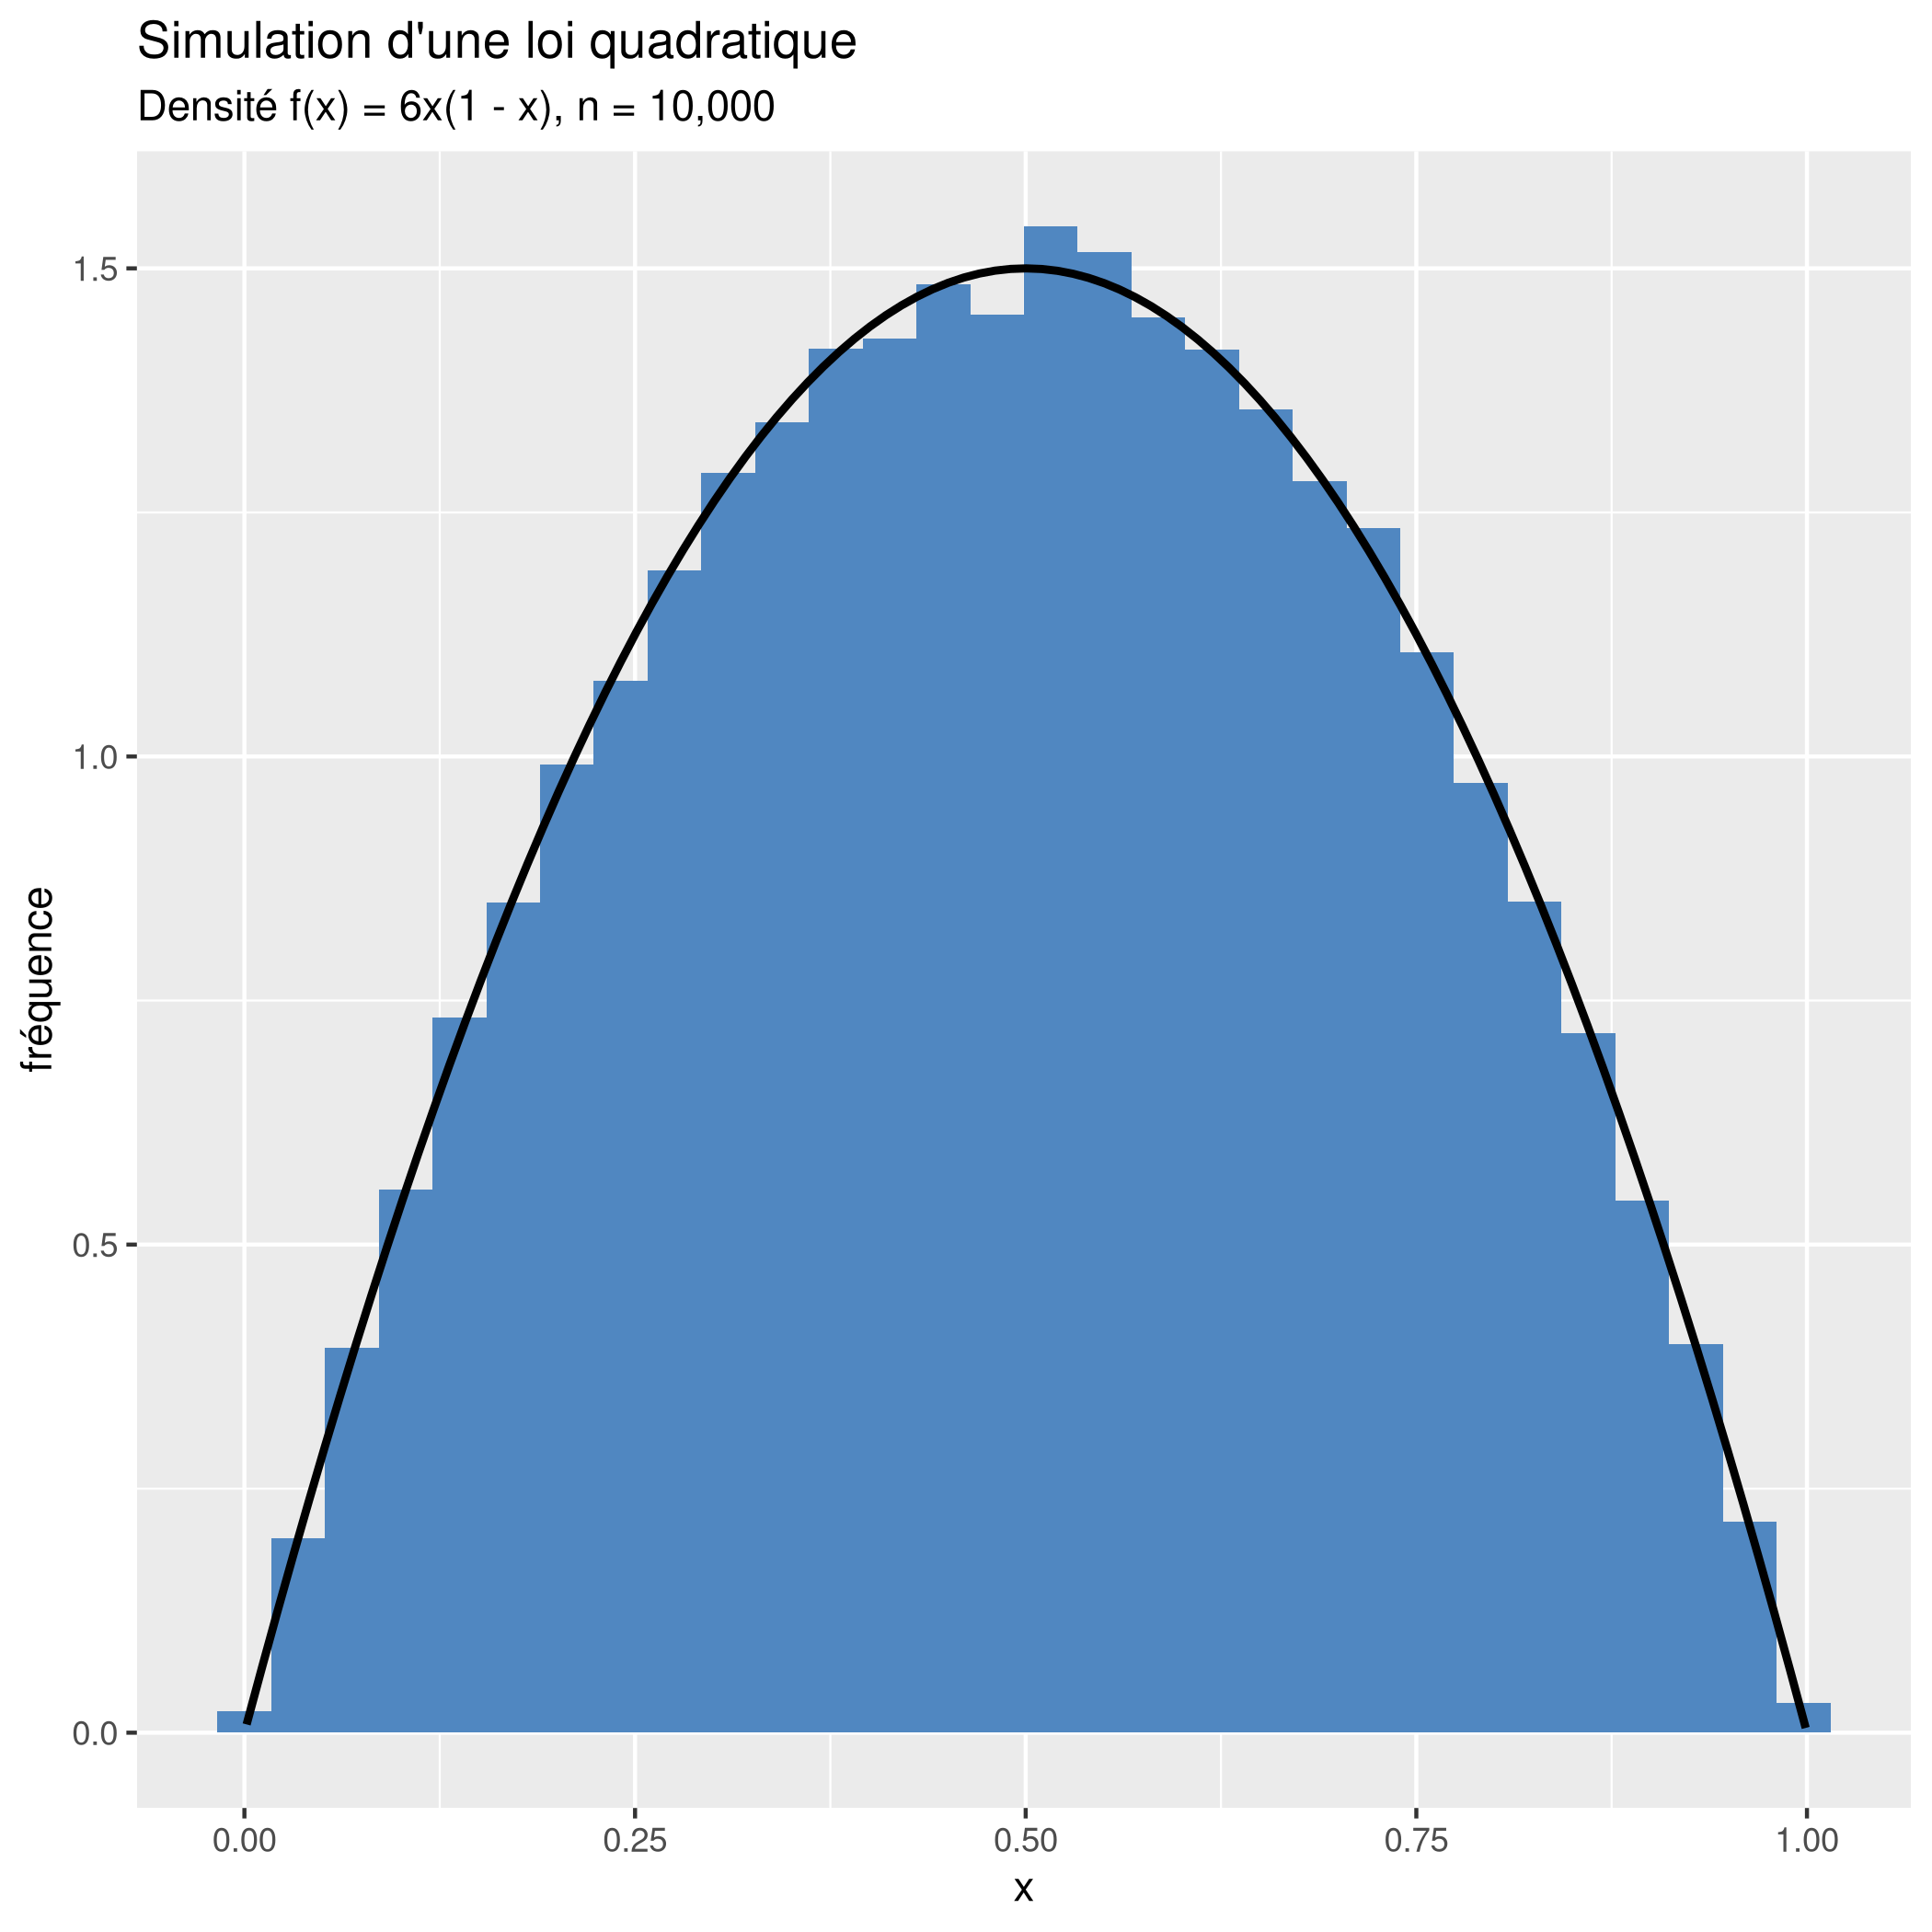
\includegraphics[width=0.6\textwidth]{media/rquad_sim.png}
    \caption{10,000 réalisations d'une variable aléatoire dont la densité est une fonction quadratique. On a vérifié graphiquement que la méthode d'acceptation-rejet implémenté en \texttt{rquad}
    permet de simuler une variable aléotoire avec $f(x) = 6x(1 - x)$.}
\end{figure}


\subsection{Loi normale}

On peut aussi appliquer la méthode d'acceptation-rejet pour simuler la loi normale. Pour rappel, la loi normale a la fonction de densité suivante :
$$f_X(x) = \frac{1}{\sigma \sqrt{2\pi}}\exp-\frac{1}{2}(\frac {x-\mu}{\sigma})^2$$

Pour ce faire, on reproduit la même méthode expliquée ci-dessus. La différence est qu'avec la loi normale, nous avons un support non compact, $  \mathbb{R} $.

Alors, nous majorons la fonction densité $f_X(x)$ en rouge de la loi normale par
$$g(x) = \left\{
    \begin{array}{ll}
        -\lambda\exp-\lambda x & \mbox{si } x \le 0 \\
        \lambda\exp-\lambda x & \mbox{sinon.}
    \end{array}
\right. $$
la densité de la loi "double exponentielle" en vert qui correspond à une variable exponentielle exp(1) affectée d'un signe positif ou négatif, tiré avec probabilité égale : 0.5.


Grâce à la méthode d'inversion, nous savons simuler des réalisations selon la loi de $g(x)$. Ces réalisations sont bien distribuées sur $  \mathbb{R} $ entier. Pour avoir une réalisation qui suit une loi normale, on commence donc par tirer X qui suit la loi de $g(x)$. Ensuite, on tire son ordonnée Y qui suit la loi $\mathcal{U}(0, g(X))$. Puis on pose une condition, si $Y > f(X)$ alors le point est rejeté, ie on ne le prend pas en compte. En revanche, si $Y \le f(X)$ alors le point est accepté. On garde uniquement sont abscisse X, qui suit alors la loi de $f_X(x)$.

\begin{figure}[h!]
\centering
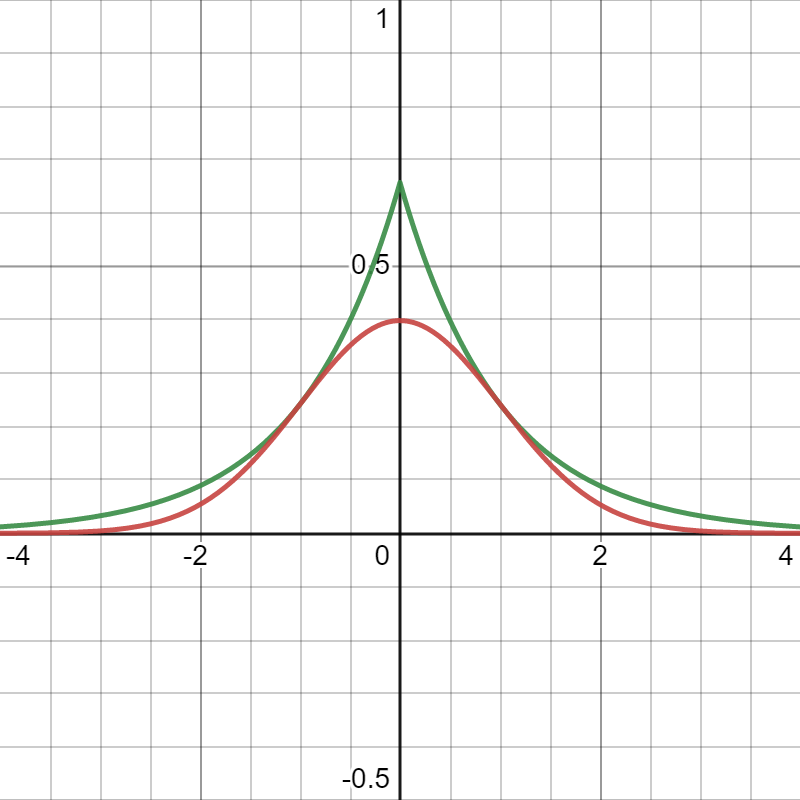
\includegraphics[scale=0.3]{media/desmos-graph.png}
\caption{Fonctions densités}
\end{figure}

On remarque que la fonction majorante en verte est extrêment serré autour de la fonction gaussienne que l'on souhaite à simuler. Plus la différence entre $f_X(x)$ et $g(x)$ est importante, plus le nombre
d'itérations qu'il faut pour accepter une valeur est grand. Cela est évident quand on considère que la probabilité d'accepter une valeur proposée est $\frac{f_X(x)}{cg(x)}$. Quand $f_X(x)$ est près de $cg(x)$,
la probabilité d'être accepté est presque 1.








On peut  implémenter l'algorithme d'acceptation-rejet pour une loi normale centrée réduite sous R :
\begin{lstlisting}[language=R]

 rnorm_acc_std <- function(n) {

    x <- vector("numeric", n)

    for (i in 1:n) {

        reject <- TRUE
        z <- 0

        while (reject) {

            y1 <- rexp(1)
            y2 <- rexp(1)

            reject <- y2 < ((y1 - 1) * (y1 - 1) / 2)

            z <- abs(y1)
        }

        if (runif(1) < 0.5) { z <- -z }
        x[[i]] <- z
    }

    x

}

\end{lstlisting}











 Par ailleurs, on peut quantifier le nombre d'itérations qu'il faut pour simuler $n$ variables aléatoirement suivant une loi normale centrée réduite.

\begin{figure}[h!]
    \centering
    % Created by tikzDevice version 0.12.3.1 on 2022-05-10 12:46:44
% !TEX encoding = UTF-8 Unicode
\begin{tikzpicture}[x=1pt,y=1pt]
\definecolor{fillColor}{RGB}{255,255,255}
\path[use as bounding box,fill=fillColor,fill opacity=0.00] (0,0) rectangle (361.35,216.81);
\begin{scope}
\path[clip] (  0.00,  0.00) rectangle (361.35,216.81);
\definecolor{drawColor}{RGB}{255,255,255}
\definecolor{fillColor}{RGB}{255,255,255}

\path[draw=drawColor,line width= 0.6pt,line join=round,line cap=round,fill=fillColor] (  0.00,  0.00) rectangle (361.35,216.81);
\end{scope}
\begin{scope}
\path[clip] ( 36.11, 30.69) rectangle (355.85,178.94);
\definecolor{fillColor}{gray}{0.92}

\path[fill=fillColor] ( 36.11, 30.69) rectangle (355.85,178.94);
\definecolor{drawColor}{RGB}{255,255,255}

\path[draw=drawColor,line width= 0.3pt,line join=round] ( 36.11, 60.78) --
	(355.85, 60.78);

\path[draw=drawColor,line width= 0.3pt,line join=round] ( 36.11,107.99) --
	(355.85,107.99);

\path[draw=drawColor,line width= 0.3pt,line join=round] ( 36.11,155.20) --
	(355.85,155.20);

\path[draw=drawColor,line width= 0.3pt,line join=round] ( 84.41, 30.69) --
	( 84.41,178.94);

\path[draw=drawColor,line width= 0.3pt,line join=round] (157.81, 30.69) --
	(157.81,178.94);

\path[draw=drawColor,line width= 0.3pt,line join=round] (231.21, 30.69) --
	(231.21,178.94);

\path[draw=drawColor,line width= 0.3pt,line join=round] (304.62, 30.69) --
	(304.62,178.94);

\path[draw=drawColor,line width= 0.6pt,line join=round] ( 36.11, 37.17) --
	(355.85, 37.17);

\path[draw=drawColor,line width= 0.6pt,line join=round] ( 36.11, 84.38) --
	(355.85, 84.38);

\path[draw=drawColor,line width= 0.6pt,line join=round] ( 36.11,131.60) --
	(355.85,131.60);

\path[draw=drawColor,line width= 0.6pt,line join=round] ( 36.11,178.81) --
	(355.85,178.81);

\path[draw=drawColor,line width= 0.6pt,line join=round] ( 47.71, 30.69) --
	( 47.71,178.94);

\path[draw=drawColor,line width= 0.6pt,line join=round] (121.11, 30.69) --
	(121.11,178.94);

\path[draw=drawColor,line width= 0.6pt,line join=round] (194.51, 30.69) --
	(194.51,178.94);

\path[draw=drawColor,line width= 0.6pt,line join=round] (267.91, 30.69) --
	(267.91,178.94);

\path[draw=drawColor,line width= 0.6pt,line join=round] (341.32, 30.69) --
	(341.32,178.94);
\definecolor{drawColor}{RGB}{0,0,0}
\definecolor{fillColor}{RGB}{0,0,0}

\path[draw=drawColor,line width= 0.4pt,line join=round,line cap=round,fill=fillColor] ( 50.64, 38.12) circle (  0.62);

\path[draw=drawColor,line width= 0.4pt,line join=round,line cap=round,fill=fillColor] ( 53.58, 39.06) circle (  0.62);

\path[draw=drawColor,line width= 0.4pt,line join=round,line cap=round,fill=fillColor] ( 56.52, 40.95) circle (  0.62);

\path[draw=drawColor,line width= 0.4pt,line join=round,line cap=round,fill=fillColor] ( 59.45, 41.89) circle (  0.62);

\path[draw=drawColor,line width= 0.4pt,line join=round,line cap=round,fill=fillColor] ( 62.39, 44.72) circle (  0.62);

\path[draw=drawColor,line width= 0.4pt,line join=round,line cap=round,fill=fillColor] ( 65.33, 43.78) circle (  0.62);

\path[draw=drawColor,line width= 0.4pt,line join=round,line cap=round,fill=fillColor] ( 68.26, 49.45) circle (  0.62);

\path[draw=drawColor,line width= 0.4pt,line join=round,line cap=round,fill=fillColor] ( 71.20, 49.45) circle (  0.62);

\path[draw=drawColor,line width= 0.4pt,line join=round,line cap=round,fill=fillColor] ( 74.13, 46.61) circle (  0.62);

\path[draw=drawColor,line width= 0.4pt,line join=round,line cap=round,fill=fillColor] ( 77.07, 46.61) circle (  0.62);

\path[draw=drawColor,line width= 0.4pt,line join=round,line cap=round,fill=fillColor] ( 80.01, 50.39) circle (  0.62);

\path[draw=drawColor,line width= 0.4pt,line join=round,line cap=round,fill=fillColor] ( 82.94, 51.33) circle (  0.62);

\path[draw=drawColor,line width= 0.4pt,line join=round,line cap=round,fill=fillColor] ( 85.88, 53.22) circle (  0.62);

\path[draw=drawColor,line width= 0.4pt,line join=round,line cap=round,fill=fillColor] ( 88.81, 53.22) circle (  0.62);

\path[draw=drawColor,line width= 0.4pt,line join=round,line cap=round,fill=fillColor] ( 91.75, 54.17) circle (  0.62);

\path[draw=drawColor,line width= 0.4pt,line join=round,line cap=round,fill=fillColor] ( 94.69, 52.28) circle (  0.62);

\path[draw=drawColor,line width= 0.4pt,line join=round,line cap=round,fill=fillColor] ( 97.62, 62.67) circle (  0.62);

\path[draw=drawColor,line width= 0.4pt,line join=round,line cap=round,fill=fillColor] (100.56, 57.00) circle (  0.62);

\path[draw=drawColor,line width= 0.4pt,line join=round,line cap=round,fill=fillColor] (103.49, 62.67) circle (  0.62);

\path[draw=drawColor,line width= 0.4pt,line join=round,line cap=round,fill=fillColor] (106.43, 62.67) circle (  0.62);

\path[draw=drawColor,line width= 0.4pt,line join=round,line cap=round,fill=fillColor] (109.37, 59.83) circle (  0.62);

\path[draw=drawColor,line width= 0.4pt,line join=round,line cap=round,fill=fillColor] (112.30, 62.67) circle (  0.62);

\path[draw=drawColor,line width= 0.4pt,line join=round,line cap=round,fill=fillColor] (115.24, 62.67) circle (  0.62);

\path[draw=drawColor,line width= 0.4pt,line join=round,line cap=round,fill=fillColor] (118.17, 67.39) circle (  0.62);

\path[draw=drawColor,line width= 0.4pt,line join=round,line cap=round,fill=fillColor] (121.11, 73.05) circle (  0.62);

\path[draw=drawColor,line width= 0.4pt,line join=round,line cap=round,fill=fillColor] (124.05, 72.11) circle (  0.62);

\path[draw=drawColor,line width= 0.4pt,line join=round,line cap=round,fill=fillColor] (126.98, 73.05) circle (  0.62);

\path[draw=drawColor,line width= 0.4pt,line join=round,line cap=round,fill=fillColor] (129.92, 81.55) circle (  0.62);

\path[draw=drawColor,line width= 0.4pt,line join=round,line cap=round,fill=fillColor] (132.85, 73.05) circle (  0.62);

\path[draw=drawColor,line width= 0.4pt,line join=round,line cap=round,fill=fillColor] (135.79, 72.11) circle (  0.62);

\path[draw=drawColor,line width= 0.4pt,line join=round,line cap=round,fill=fillColor] (138.73, 72.11) circle (  0.62);

\path[draw=drawColor,line width= 0.4pt,line join=round,line cap=round,fill=fillColor] (141.66, 82.50) circle (  0.62);

\path[draw=drawColor,line width= 0.4pt,line join=round,line cap=round,fill=fillColor] (144.60, 75.89) circle (  0.62);

\path[draw=drawColor,line width= 0.4pt,line join=round,line cap=round,fill=fillColor] (147.54, 81.55) circle (  0.62);

\path[draw=drawColor,line width= 0.4pt,line join=round,line cap=round,fill=fillColor] (150.47, 84.38) circle (  0.62);

\path[draw=drawColor,line width= 0.4pt,line join=round,line cap=round,fill=fillColor] (153.41, 84.38) circle (  0.62);

\path[draw=drawColor,line width= 0.4pt,line join=round,line cap=round,fill=fillColor] (156.34, 85.33) circle (  0.62);

\path[draw=drawColor,line width= 0.4pt,line join=round,line cap=round,fill=fillColor] (159.28, 80.61) circle (  0.62);

\path[draw=drawColor,line width= 0.4pt,line join=round,line cap=round,fill=fillColor] (162.22, 87.22) circle (  0.62);

\path[draw=drawColor,line width= 0.4pt,line join=round,line cap=round,fill=fillColor] (165.15, 77.77) circle (  0.62);

\path[draw=drawColor,line width= 0.4pt,line join=round,line cap=round,fill=fillColor] (168.09, 86.27) circle (  0.62);

\path[draw=drawColor,line width= 0.4pt,line join=round,line cap=round,fill=fillColor] (171.02, 88.16) circle (  0.62);

\path[draw=drawColor,line width= 0.4pt,line join=round,line cap=round,fill=fillColor] (173.96, 90.05) circle (  0.62);

\path[draw=drawColor,line width= 0.4pt,line join=round,line cap=round,fill=fillColor] (176.90, 86.27) circle (  0.62);

\path[draw=drawColor,line width= 0.4pt,line join=round,line cap=round,fill=fillColor] (179.83, 92.88) circle (  0.62);

\path[draw=drawColor,line width= 0.4pt,line join=round,line cap=round,fill=fillColor] (182.77, 93.83) circle (  0.62);

\path[draw=drawColor,line width= 0.4pt,line join=round,line cap=round,fill=fillColor] (185.70, 90.99) circle (  0.62);

\path[draw=drawColor,line width= 0.4pt,line join=round,line cap=round,fill=fillColor] (188.64, 90.99) circle (  0.62);

\path[draw=drawColor,line width= 0.4pt,line join=round,line cap=round,fill=fillColor] (191.58,100.44) circle (  0.62);

\path[draw=drawColor,line width= 0.4pt,line join=round,line cap=round,fill=fillColor] (194.51,104.21) circle (  0.62);

\path[draw=drawColor,line width= 0.4pt,line join=round,line cap=round,fill=fillColor] (197.45,101.38) circle (  0.62);

\path[draw=drawColor,line width= 0.4pt,line join=round,line cap=round,fill=fillColor] (200.38,105.16) circle (  0.62);

\path[draw=drawColor,line width= 0.4pt,line join=round,line cap=round,fill=fillColor] (203.32, 93.83) circle (  0.62);

\path[draw=drawColor,line width= 0.4pt,line join=round,line cap=round,fill=fillColor] (206.26,102.32) circle (  0.62);

\path[draw=drawColor,line width= 0.4pt,line join=round,line cap=round,fill=fillColor] (209.19, 98.55) circle (  0.62);

\path[draw=drawColor,line width= 0.4pt,line join=round,line cap=round,fill=fillColor] (212.13,106.10) circle (  0.62);

\path[draw=drawColor,line width= 0.4pt,line join=round,line cap=round,fill=fillColor] (215.07,112.71) circle (  0.62);

\path[draw=drawColor,line width= 0.4pt,line join=round,line cap=round,fill=fillColor] (218.00,108.93) circle (  0.62);

\path[draw=drawColor,line width= 0.4pt,line join=round,line cap=round,fill=fillColor] (220.94,107.05) circle (  0.62);

\path[draw=drawColor,line width= 0.4pt,line join=round,line cap=round,fill=fillColor] (223.87,109.88) circle (  0.62);

\path[draw=drawColor,line width= 0.4pt,line join=round,line cap=round,fill=fillColor] (226.81,114.60) circle (  0.62);

\path[draw=drawColor,line width= 0.4pt,line join=round,line cap=round,fill=fillColor] (229.75,114.60) circle (  0.62);

\path[draw=drawColor,line width= 0.4pt,line join=round,line cap=round,fill=fillColor] (232.68,109.88) circle (  0.62);

\path[draw=drawColor,line width= 0.4pt,line join=round,line cap=round,fill=fillColor] (235.62,121.21) circle (  0.62);

\path[draw=drawColor,line width= 0.4pt,line join=round,line cap=round,fill=fillColor] (238.55,111.77) circle (  0.62);

\path[draw=drawColor,line width= 0.4pt,line join=round,line cap=round,fill=fillColor] (241.49,117.43) circle (  0.62);

\path[draw=drawColor,line width= 0.4pt,line join=round,line cap=round,fill=fillColor] (244.43,131.60) circle (  0.62);

\path[draw=drawColor,line width= 0.4pt,line join=round,line cap=round,fill=fillColor] (247.36,120.27) circle (  0.62);

\path[draw=drawColor,line width= 0.4pt,line join=round,line cap=round,fill=fillColor] (250.30,123.10) circle (  0.62);

\path[draw=drawColor,line width= 0.4pt,line join=round,line cap=round,fill=fillColor] (253.23,130.65) circle (  0.62);

\path[draw=drawColor,line width= 0.4pt,line join=round,line cap=round,fill=fillColor] (256.17,121.21) circle (  0.62);

\path[draw=drawColor,line width= 0.4pt,line join=round,line cap=round,fill=fillColor] (259.11,126.88) circle (  0.62);

\path[draw=drawColor,line width= 0.4pt,line join=round,line cap=round,fill=fillColor] (262.04,127.82) circle (  0.62);

\path[draw=drawColor,line width= 0.4pt,line join=round,line cap=round,fill=fillColor] (264.98,131.60) circle (  0.62);

\path[draw=drawColor,line width= 0.4pt,line join=round,line cap=round,fill=fillColor] (267.91,122.15) circle (  0.62);

\path[draw=drawColor,line width= 0.4pt,line join=round,line cap=round,fill=fillColor] (270.85,136.32) circle (  0.62);

\path[draw=drawColor,line width= 0.4pt,line join=round,line cap=round,fill=fillColor] (273.79,145.76) circle (  0.62);

\path[draw=drawColor,line width= 0.4pt,line join=round,line cap=round,fill=fillColor] (276.72,138.21) circle (  0.62);

\path[draw=drawColor,line width= 0.4pt,line join=round,line cap=round,fill=fillColor] (279.66,134.43) circle (  0.62);

\path[draw=drawColor,line width= 0.4pt,line join=round,line cap=round,fill=fillColor] (282.59,138.21) circle (  0.62);

\path[draw=drawColor,line width= 0.4pt,line join=round,line cap=round,fill=fillColor] (285.53,128.76) circle (  0.62);

\path[draw=drawColor,line width= 0.4pt,line join=round,line cap=round,fill=fillColor] (288.47,141.04) circle (  0.62);

\path[draw=drawColor,line width= 0.4pt,line join=round,line cap=round,fill=fillColor] (291.40,141.98) circle (  0.62);

\path[draw=drawColor,line width= 0.4pt,line join=round,line cap=round,fill=fillColor] (294.34,142.93) circle (  0.62);

\path[draw=drawColor,line width= 0.4pt,line join=round,line cap=round,fill=fillColor] (297.28,134.43) circle (  0.62);

\path[draw=drawColor,line width= 0.4pt,line join=round,line cap=round,fill=fillColor] (300.21,158.04) circle (  0.62);

\path[draw=drawColor,line width= 0.4pt,line join=round,line cap=round,fill=fillColor] (303.15,150.48) circle (  0.62);

\path[draw=drawColor,line width= 0.4pt,line join=round,line cap=round,fill=fillColor] (306.08,150.48) circle (  0.62);

\path[draw=drawColor,line width= 0.4pt,line join=round,line cap=round,fill=fillColor] (309.02,151.43) circle (  0.62);

\path[draw=drawColor,line width= 0.4pt,line join=round,line cap=round,fill=fillColor] (311.96,150.48) circle (  0.62);

\path[draw=drawColor,line width= 0.4pt,line join=round,line cap=round,fill=fillColor] (314.89,155.20) circle (  0.62);

\path[draw=drawColor,line width= 0.4pt,line join=round,line cap=round,fill=fillColor] (317.83,148.59) circle (  0.62);

\path[draw=drawColor,line width= 0.4pt,line join=round,line cap=round,fill=fillColor] (320.76,158.04) circle (  0.62);

\path[draw=drawColor,line width= 0.4pt,line join=round,line cap=round,fill=fillColor] (323.70,154.26) circle (  0.62);

\path[draw=drawColor,line width= 0.4pt,line join=round,line cap=round,fill=fillColor] (326.64,148.59) circle (  0.62);

\path[draw=drawColor,line width= 0.4pt,line join=round,line cap=round,fill=fillColor] (329.57,149.54) circle (  0.62);

\path[draw=drawColor,line width= 0.4pt,line join=round,line cap=round,fill=fillColor] (332.51,160.87) circle (  0.62);

\path[draw=drawColor,line width= 0.4pt,line join=round,line cap=round,fill=fillColor] (335.44,169.37) circle (  0.62);

\path[draw=drawColor,line width= 0.4pt,line join=round,line cap=round,fill=fillColor] (338.38,172.20) circle (  0.62);

\path[draw=drawColor,line width= 0.4pt,line join=round,line cap=round,fill=fillColor] (341.32,165.59) circle (  0.62);

\path[draw=drawColor,line width= 0.3pt,line join=round] ( 50.64, 37.42) --
	( 53.58, 38.69) --
	( 56.52, 39.96) --
	( 59.45, 41.23) --
	( 62.39, 42.50) --
	( 65.33, 43.78) --
	( 68.26, 45.05) --
	( 71.20, 46.32) --
	( 74.13, 47.59) --
	( 77.07, 48.86) --
	( 80.01, 50.13) --
	( 82.94, 51.40) --
	( 85.88, 52.67) --
	( 88.81, 53.94) --
	( 91.75, 55.21) --
	( 94.69, 56.48) --
	( 97.62, 57.75) --
	(100.56, 59.02) --
	(103.49, 60.29) --
	(106.43, 61.56) --
	(109.37, 62.83) --
	(112.30, 64.10) --
	(115.24, 65.37) --
	(118.17, 66.64) --
	(121.11, 67.91) --
	(124.05, 69.18) --
	(126.98, 70.45) --
	(129.92, 71.72) --
	(132.85, 72.99) --
	(135.79, 74.26) --
	(138.73, 75.53) --
	(141.66, 76.80) --
	(144.60, 78.07) --
	(147.54, 79.34) --
	(150.47, 80.61) --
	(153.41, 81.88) --
	(156.34, 83.15) --
	(159.28, 84.42) --
	(162.22, 85.69) --
	(165.15, 86.96) --
	(168.09, 88.23) --
	(171.02, 89.50) --
	(173.96, 90.77) --
	(176.90, 92.04) --
	(179.83, 93.31) --
	(182.77, 94.58) --
	(185.70, 95.85) --
	(188.64, 97.12) --
	(191.58, 98.39) --
	(194.51, 99.66) --
	(197.45,100.93) --
	(200.38,102.20) --
	(203.32,103.47) --
	(206.26,104.74) --
	(209.19,106.01) --
	(212.13,107.28) --
	(215.07,108.55) --
	(218.00,109.82) --
	(220.94,111.09) --
	(223.87,112.36) --
	(226.81,113.63) --
	(229.75,114.90) --
	(232.68,116.17) --
	(235.62,117.44) --
	(238.55,118.71) --
	(241.49,119.98) --
	(244.43,121.25) --
	(247.36,122.52) --
	(250.30,123.79) --
	(253.23,125.06) --
	(256.17,126.33) --
	(259.11,127.60) --
	(262.04,128.87) --
	(264.98,130.14) --
	(267.91,131.41) --
	(270.85,132.68) --
	(273.79,133.95) --
	(276.72,135.22) --
	(279.66,136.49) --
	(282.59,137.76) --
	(285.53,139.03) --
	(288.47,140.30) --
	(291.40,141.57) --
	(294.34,142.84) --
	(297.28,144.11) --
	(300.21,145.38) --
	(303.15,146.65) --
	(306.08,147.92) --
	(309.02,149.19) --
	(311.96,150.46) --
	(314.89,151.73) --
	(317.83,153.00) --
	(320.76,154.27) --
	(323.70,155.54) --
	(326.64,156.81) --
	(329.57,158.08) --
	(332.51,159.35) --
	(335.44,160.62) --
	(338.38,161.89) --
	(341.32,163.16);
\definecolor{drawColor}{RGB}{255,0,0}

\path[draw=drawColor,draw opacity=0.30,line width= 0.6pt,line join=round] ( 50.64, 37.42) --
	( 53.58, 38.69) --
	( 56.52, 39.96) --
	( 59.45, 41.23) --
	( 62.39, 42.50) --
	( 65.33, 43.78) --
	( 68.26, 45.05) --
	( 71.20, 46.32) --
	( 74.13, 47.59) --
	( 77.07, 48.86) --
	( 80.01, 50.13) --
	( 82.94, 51.40) --
	( 85.88, 52.67) --
	( 88.81, 53.94) --
	( 91.75, 55.21) --
	( 94.69, 56.48) --
	( 97.62, 57.75) --
	(100.56, 59.02) --
	(103.49, 60.29) --
	(106.43, 61.56) --
	(109.37, 62.83) --
	(112.30, 64.10) --
	(115.24, 65.37) --
	(118.17, 66.64) --
	(121.11, 67.91) --
	(124.05, 69.18) --
	(126.98, 70.45) --
	(129.92, 71.72) --
	(132.85, 72.99) --
	(135.79, 74.26) --
	(138.73, 75.53) --
	(141.66, 76.80) --
	(144.60, 78.07) --
	(147.54, 79.34) --
	(150.47, 80.61) --
	(153.41, 81.88) --
	(156.34, 83.15) --
	(159.28, 84.42) --
	(162.22, 85.69) --
	(165.15, 86.96) --
	(168.09, 88.23) --
	(171.02, 89.50) --
	(173.96, 90.77) --
	(176.90, 92.04) --
	(179.83, 93.31) --
	(182.77, 94.58) --
	(185.70, 95.85) --
	(188.64, 97.12) --
	(191.58, 98.39) --
	(194.51, 99.66) --
	(197.45,100.93) --
	(200.38,102.20) --
	(203.32,103.47) --
	(206.26,104.74) --
	(209.19,106.01) --
	(212.13,107.28) --
	(215.07,108.55) --
	(218.00,109.82) --
	(220.94,111.09) --
	(223.87,112.36) --
	(226.81,113.63) --
	(229.75,114.90) --
	(232.68,116.17) --
	(235.62,117.44) --
	(238.55,118.71) --
	(241.49,119.98) --
	(244.43,121.25) --
	(247.36,122.52) --
	(250.30,123.79) --
	(253.23,125.06) --
	(256.17,126.33) --
	(259.11,127.60) --
	(262.04,128.87) --
	(264.98,130.14) --
	(267.91,131.41) --
	(270.85,132.68) --
	(273.79,133.95) --
	(276.72,135.22) --
	(279.66,136.49) --
	(282.59,137.76) --
	(285.53,139.03) --
	(288.47,140.30) --
	(291.40,141.57) --
	(294.34,142.84) --
	(297.28,144.11) --
	(300.21,145.38) --
	(303.15,146.65) --
	(306.08,147.92) --
	(309.02,149.19) --
	(311.96,150.46) --
	(314.89,151.73) --
	(317.83,153.00) --
	(320.76,154.27) --
	(323.70,155.54) --
	(326.64,156.81) --
	(329.57,158.08) --
	(332.51,159.35) --
	(335.44,160.62) --
	(338.38,161.89) --
	(341.32,163.16);
\definecolor{drawColor}{RGB}{255,0,0}

\path[draw=drawColor,line width= 0.6pt,line join=round] ( 50.64, 37.42) -- ( 50.64, 38.12);

\path[draw=drawColor,line width= 0.6pt,line join=round] ( 53.58, 38.69) -- ( 53.58, 39.06);

\path[draw=drawColor,line width= 0.6pt,line join=round] ( 56.52, 39.96) -- ( 56.52, 40.95);

\path[draw=drawColor,line width= 0.6pt,line join=round] ( 59.45, 41.23) -- ( 59.45, 41.89);

\path[draw=drawColor,line width= 0.6pt,line join=round] ( 62.39, 42.50) -- ( 62.39, 44.72);

\path[draw=drawColor,line width= 0.6pt,line join=round] ( 65.33, 43.78) -- ( 65.33, 43.78);

\path[draw=drawColor,line width= 0.6pt,line join=round] ( 68.26, 45.05) -- ( 68.26, 49.45);

\path[draw=drawColor,line width= 0.6pt,line join=round] ( 71.20, 46.32) -- ( 71.20, 49.45);

\path[draw=drawColor,line width= 0.6pt,line join=round] ( 74.13, 47.59) -- ( 74.13, 46.61);

\path[draw=drawColor,line width= 0.6pt,line join=round] ( 77.07, 48.86) -- ( 77.07, 46.61);

\path[draw=drawColor,line width= 0.6pt,line join=round] ( 80.01, 50.13) -- ( 80.01, 50.39);

\path[draw=drawColor,line width= 0.6pt,line join=round] ( 82.94, 51.40) -- ( 82.94, 51.33);

\path[draw=drawColor,line width= 0.6pt,line join=round] ( 85.88, 52.67) -- ( 85.88, 53.22);

\path[draw=drawColor,line width= 0.6pt,line join=round] ( 88.81, 53.94) -- ( 88.81, 53.22);

\path[draw=drawColor,line width= 0.6pt,line join=round] ( 91.75, 55.21) -- ( 91.75, 54.17);

\path[draw=drawColor,line width= 0.6pt,line join=round] ( 94.69, 56.48) -- ( 94.69, 52.28);

\path[draw=drawColor,line width= 0.6pt,line join=round] ( 97.62, 57.75) -- ( 97.62, 62.67);

\path[draw=drawColor,line width= 0.6pt,line join=round] (100.56, 59.02) -- (100.56, 57.00);

\path[draw=drawColor,line width= 0.6pt,line join=round] (103.49, 60.29) -- (103.49, 62.67);

\path[draw=drawColor,line width= 0.6pt,line join=round] (106.43, 61.56) -- (106.43, 62.67);

\path[draw=drawColor,line width= 0.6pt,line join=round] (109.37, 62.83) -- (109.37, 59.83);

\path[draw=drawColor,line width= 0.6pt,line join=round] (112.30, 64.10) -- (112.30, 62.67);

\path[draw=drawColor,line width= 0.6pt,line join=round] (115.24, 65.37) -- (115.24, 62.67);

\path[draw=drawColor,line width= 0.6pt,line join=round] (118.17, 66.64) -- (118.17, 67.39);

\path[draw=drawColor,line width= 0.6pt,line join=round] (121.11, 67.91) -- (121.11, 73.05);

\path[draw=drawColor,line width= 0.6pt,line join=round] (124.05, 69.18) -- (124.05, 72.11);

\path[draw=drawColor,line width= 0.6pt,line join=round] (126.98, 70.45) -- (126.98, 73.05);

\path[draw=drawColor,line width= 0.6pt,line join=round] (129.92, 71.72) -- (129.92, 81.55);

\path[draw=drawColor,line width= 0.6pt,line join=round] (132.85, 72.99) -- (132.85, 73.05);

\path[draw=drawColor,line width= 0.6pt,line join=round] (135.79, 74.26) -- (135.79, 72.11);

\path[draw=drawColor,line width= 0.6pt,line join=round] (138.73, 75.53) -- (138.73, 72.11);

\path[draw=drawColor,line width= 0.6pt,line join=round] (141.66, 76.80) -- (141.66, 82.50);

\path[draw=drawColor,line width= 0.6pt,line join=round] (144.60, 78.07) -- (144.60, 75.89);

\path[draw=drawColor,line width= 0.6pt,line join=round] (147.54, 79.34) -- (147.54, 81.55);

\path[draw=drawColor,line width= 0.6pt,line join=round] (150.47, 80.61) -- (150.47, 84.38);

\path[draw=drawColor,line width= 0.6pt,line join=round] (153.41, 81.88) -- (153.41, 84.38);

\path[draw=drawColor,line width= 0.6pt,line join=round] (156.34, 83.15) -- (156.34, 85.33);

\path[draw=drawColor,line width= 0.6pt,line join=round] (159.28, 84.42) -- (159.28, 80.61);

\path[draw=drawColor,line width= 0.6pt,line join=round] (162.22, 85.69) -- (162.22, 87.22);

\path[draw=drawColor,line width= 0.6pt,line join=round] (165.15, 86.96) -- (165.15, 77.77);

\path[draw=drawColor,line width= 0.6pt,line join=round] (168.09, 88.23) -- (168.09, 86.27);

\path[draw=drawColor,line width= 0.6pt,line join=round] (171.02, 89.50) -- (171.02, 88.16);

\path[draw=drawColor,line width= 0.6pt,line join=round] (173.96, 90.77) -- (173.96, 90.05);

\path[draw=drawColor,line width= 0.6pt,line join=round] (176.90, 92.04) -- (176.90, 86.27);

\path[draw=drawColor,line width= 0.6pt,line join=round] (179.83, 93.31) -- (179.83, 92.88);

\path[draw=drawColor,line width= 0.6pt,line join=round] (182.77, 94.58) -- (182.77, 93.83);

\path[draw=drawColor,line width= 0.6pt,line join=round] (185.70, 95.85) -- (185.70, 90.99);

\path[draw=drawColor,line width= 0.6pt,line join=round] (188.64, 97.12) -- (188.64, 90.99);

\path[draw=drawColor,line width= 0.6pt,line join=round] (191.58, 98.39) -- (191.58,100.44);

\path[draw=drawColor,line width= 0.6pt,line join=round] (194.51, 99.66) -- (194.51,104.21);

\path[draw=drawColor,line width= 0.6pt,line join=round] (197.45,100.93) -- (197.45,101.38);

\path[draw=drawColor,line width= 0.6pt,line join=round] (200.38,102.20) -- (200.38,105.16);

\path[draw=drawColor,line width= 0.6pt,line join=round] (203.32,103.47) -- (203.32, 93.83);

\path[draw=drawColor,line width= 0.6pt,line join=round] (206.26,104.74) -- (206.26,102.32);

\path[draw=drawColor,line width= 0.6pt,line join=round] (209.19,106.01) -- (209.19, 98.55);

\path[draw=drawColor,line width= 0.6pt,line join=round] (212.13,107.28) -- (212.13,106.10);

\path[draw=drawColor,line width= 0.6pt,line join=round] (215.07,108.55) -- (215.07,112.71);

\path[draw=drawColor,line width= 0.6pt,line join=round] (218.00,109.82) -- (218.00,108.93);

\path[draw=drawColor,line width= 0.6pt,line join=round] (220.94,111.09) -- (220.94,107.05);

\path[draw=drawColor,line width= 0.6pt,line join=round] (223.87,112.36) -- (223.87,109.88);

\path[draw=drawColor,line width= 0.6pt,line join=round] (226.81,113.63) -- (226.81,114.60);

\path[draw=drawColor,line width= 0.6pt,line join=round] (229.75,114.90) -- (229.75,114.60);

\path[draw=drawColor,line width= 0.6pt,line join=round] (232.68,116.17) -- (232.68,109.88);

\path[draw=drawColor,line width= 0.6pt,line join=round] (235.62,117.44) -- (235.62,121.21);

\path[draw=drawColor,line width= 0.6pt,line join=round] (238.55,118.71) -- (238.55,111.77);

\path[draw=drawColor,line width= 0.6pt,line join=round] (241.49,119.98) -- (241.49,117.43);

\path[draw=drawColor,line width= 0.6pt,line join=round] (244.43,121.25) -- (244.43,131.60);

\path[draw=drawColor,line width= 0.6pt,line join=round] (247.36,122.52) -- (247.36,120.27);

\path[draw=drawColor,line width= 0.6pt,line join=round] (250.30,123.79) -- (250.30,123.10);

\path[draw=drawColor,line width= 0.6pt,line join=round] (253.23,125.06) -- (253.23,130.65);

\path[draw=drawColor,line width= 0.6pt,line join=round] (256.17,126.33) -- (256.17,121.21);

\path[draw=drawColor,line width= 0.6pt,line join=round] (259.11,127.60) -- (259.11,126.88);

\path[draw=drawColor,line width= 0.6pt,line join=round] (262.04,128.87) -- (262.04,127.82);

\path[draw=drawColor,line width= 0.6pt,line join=round] (264.98,130.14) -- (264.98,131.60);

\path[draw=drawColor,line width= 0.6pt,line join=round] (267.91,131.41) -- (267.91,122.15);

\path[draw=drawColor,line width= 0.6pt,line join=round] (270.85,132.68) -- (270.85,136.32);

\path[draw=drawColor,line width= 0.6pt,line join=round] (273.79,133.95) -- (273.79,145.76);

\path[draw=drawColor,line width= 0.6pt,line join=round] (276.72,135.22) -- (276.72,138.21);

\path[draw=drawColor,line width= 0.6pt,line join=round] (279.66,136.49) -- (279.66,134.43);

\path[draw=drawColor,line width= 0.6pt,line join=round] (282.59,137.76) -- (282.59,138.21);

\path[draw=drawColor,line width= 0.6pt,line join=round] (285.53,139.03) -- (285.53,128.76);

\path[draw=drawColor,line width= 0.6pt,line join=round] (288.47,140.30) -- (288.47,141.04);

\path[draw=drawColor,line width= 0.6pt,line join=round] (291.40,141.57) -- (291.40,141.98);

\path[draw=drawColor,line width= 0.6pt,line join=round] (294.34,142.84) -- (294.34,142.93);

\path[draw=drawColor,line width= 0.6pt,line join=round] (297.28,144.11) -- (297.28,134.43);

\path[draw=drawColor,line width= 0.6pt,line join=round] (300.21,145.38) -- (300.21,158.04);

\path[draw=drawColor,line width= 0.6pt,line join=round] (303.15,146.65) -- (303.15,150.48);

\path[draw=drawColor,line width= 0.6pt,line join=round] (306.08,147.92) -- (306.08,150.48);

\path[draw=drawColor,line width= 0.6pt,line join=round] (309.02,149.19) -- (309.02,151.43);

\path[draw=drawColor,line width= 0.6pt,line join=round] (311.96,150.46) -- (311.96,150.48);

\path[draw=drawColor,line width= 0.6pt,line join=round] (314.89,151.73) -- (314.89,155.20);

\path[draw=drawColor,line width= 0.6pt,line join=round] (317.83,153.00) -- (317.83,148.59);

\path[draw=drawColor,line width= 0.6pt,line join=round] (320.76,154.27) -- (320.76,158.04);

\path[draw=drawColor,line width= 0.6pt,line join=round] (323.70,155.54) -- (323.70,154.26);

\path[draw=drawColor,line width= 0.6pt,line join=round] (326.64,156.81) -- (326.64,148.59);

\path[draw=drawColor,line width= 0.6pt,line join=round] (329.57,158.08) -- (329.57,149.54);

\path[draw=drawColor,line width= 0.6pt,line join=round] (332.51,159.35) -- (332.51,160.87);

\path[draw=drawColor,line width= 0.6pt,line join=round] (335.44,160.62) -- (335.44,169.37);

\path[draw=drawColor,line width= 0.6pt,line join=round] (338.38,161.89) -- (338.38,172.20);

\path[draw=drawColor,line width= 0.6pt,line join=round] (341.32,163.16) -- (341.32,165.59);
\end{scope}
\begin{scope}
\path[clip] (  0.00,  0.00) rectangle (361.35,216.81);
\definecolor{drawColor}{gray}{0.30}

\node[text=drawColor,anchor=base east,inner sep=0pt, outer sep=0pt, scale=  0.88] at ( 31.16, 34.14) {0};

\node[text=drawColor,anchor=base east,inner sep=0pt, outer sep=0pt, scale=  0.88] at ( 31.16, 81.35) {50};

\node[text=drawColor,anchor=base east,inner sep=0pt, outer sep=0pt, scale=  0.88] at ( 31.16,128.57) {100};

\node[text=drawColor,anchor=base east,inner sep=0pt, outer sep=0pt, scale=  0.88] at ( 31.16,175.78) {150};
\end{scope}
\begin{scope}
\path[clip] (  0.00,  0.00) rectangle (361.35,216.81);
\definecolor{drawColor}{gray}{0.20}

\path[draw=drawColor,line width= 0.6pt,line join=round] ( 33.36, 37.17) --
	( 36.11, 37.17);

\path[draw=drawColor,line width= 0.6pt,line join=round] ( 33.36, 84.38) --
	( 36.11, 84.38);

\path[draw=drawColor,line width= 0.6pt,line join=round] ( 33.36,131.60) --
	( 36.11,131.60);

\path[draw=drawColor,line width= 0.6pt,line join=round] ( 33.36,178.81) --
	( 36.11,178.81);
\end{scope}
\begin{scope}
\path[clip] (  0.00,  0.00) rectangle (361.35,216.81);
\definecolor{drawColor}{gray}{0.20}

\path[draw=drawColor,line width= 0.6pt,line join=round] ( 47.71, 27.94) --
	( 47.71, 30.69);

\path[draw=drawColor,line width= 0.6pt,line join=round] (121.11, 27.94) --
	(121.11, 30.69);

\path[draw=drawColor,line width= 0.6pt,line join=round] (194.51, 27.94) --
	(194.51, 30.69);

\path[draw=drawColor,line width= 0.6pt,line join=round] (267.91, 27.94) --
	(267.91, 30.69);

\path[draw=drawColor,line width= 0.6pt,line join=round] (341.32, 27.94) --
	(341.32, 30.69);
\end{scope}
\begin{scope}
\path[clip] (  0.00,  0.00) rectangle (361.35,216.81);
\definecolor{drawColor}{gray}{0.30}

\node[text=drawColor,anchor=base,inner sep=0pt, outer sep=0pt, scale=  0.88] at ( 47.71, 19.68) {0};

\node[text=drawColor,anchor=base,inner sep=0pt, outer sep=0pt, scale=  0.88] at (121.11, 19.68) {25};

\node[text=drawColor,anchor=base,inner sep=0pt, outer sep=0pt, scale=  0.88] at (194.51, 19.68) {50};

\node[text=drawColor,anchor=base,inner sep=0pt, outer sep=0pt, scale=  0.88] at (267.91, 19.68) {75};

\node[text=drawColor,anchor=base,inner sep=0pt, outer sep=0pt, scale=  0.88] at (341.32, 19.68) {100};
\end{scope}
\begin{scope}
\path[clip] (  0.00,  0.00) rectangle (361.35,216.81);
\definecolor{drawColor}{RGB}{0,0,0}

\node[text=drawColor,anchor=base,inner sep=0pt, outer sep=0pt, scale=  1.10] at (195.98,  7.64) {$n$};
\end{scope}
\begin{scope}
\path[clip] (  0.00,  0.00) rectangle (361.35,216.81);
\definecolor{drawColor}{RGB}{0,0,0}

\node[text=drawColor,rotate= 90.00,anchor=base,inner sep=0pt, outer sep=0pt, scale=  1.10] at ( 13.08,104.81) {$\texttt{nrej}(n) \approx 1.35n$};
\end{scope}
\begin{scope}
\path[clip] (  0.00,  0.00) rectangle (361.35,216.81);
\definecolor{drawColor}{RGB}{0,0,0}

\node[text=drawColor,anchor=base west,inner sep=0pt, outer sep=0pt, scale=  1.10] at ( 36.11,186.58) {Pour n realisations d'une variable aleatoire normale};
\end{scope}
\begin{scope}
\path[clip] (  0.00,  0.00) rectangle (361.35,216.81);
\definecolor{drawColor}{RGB}{0,0,0}

\node[text=drawColor,anchor=base west,inner sep=0pt, outer sep=0pt, scale=  1.32] at ( 36.11,202.22) {Moyenne des rejections};
\end{scope}
\end{tikzpicture}

    \caption{Moyenne des rejets}
\end{figure}
%%wtf comment on change le titre


La pente de cette courbe représente le pourcentage de variables simulées totales sur le nombre de variable acceptées. Ce pourcentage vaut environ 1,35 c'est-à-dire que pour simuler 100 variables, il faudra en moyenne en tirer 135 en tout. Ce chiffre est spécifique au coeficient que nous avons choisi pour la fonction majorante $g(x)$

%% on pourrait mettre 1 comme coef devant g(x) au lieu de sqrt(1/2e) et montrez que la pente est grave supérieure


\subsection{Box-Muller}

La loi normale n’a pas une densité à support compact et on ne connaît pas d’expression simple de l’inverse de sa
fonction de répartition. On ne peut donc, théoriquement, employer la méthode de transformation inversée. On présente
ici une méthode qui permet de simuler un couple des variables aléatoires normales, centrées, réduites et indépendantes.
On veut simuler $X \sim \mathcal{N} (0, 1)$ et $Y \sim \mathcal{N} (0, 1)$ indépendantes. On connaît la densité jointe de $X$ et
 $Y$ :

$$f_X,_Y(x,y) = \frac{1}{2\pi}\exp(-\frac {x^2+y^2}{2})$$

On effectue le passage en coordonnées polaires

$$x = \rho \cos(\theta), y = \rho \sin(\theta)$$

et on obtient

$$f_X,_Y(x,y)dxdy = \frac {1}{2\pi}\exp(-\frac {\rho^2}{2})\rho d\rho d\theta = f_R,_\theta(\rho,\theta)d\rho d\theta$$

Dans la densité jointe des variable $R$ et $\theta$, on reconnaît

$\frac{1}{2\pi} =$ densité de $\theta$ qui suit une loi Uniforme sur 0 et 2 $\pi$.


$\rho \exp(-\frac{\rho^2}{2}) = $densité de R.

On en déduit la fonction de répartition de R :

$$F_R(\rho) = 1- exp(-\frac{t^2}{2})$$

On reconnaît une loi exponentielle de paramètres 1/2 pour $R^2$.\\
On a donc les lois de $R$ et  $\theta$ :

$$R^2 ~ \exp(\frac{1}{2}), \theta ~ U([0, 2\pi])$$

La méthode consiste donc à tirer deux variables uniforme $U_1$ et $U_2$, puis on insère ces deux variables dans les formule suivante: \\

$$R = \sqrt{-2 \ln U_1}$$

$$\theta = 2\pi U_2$$

et on pose :

$$X = R\cos\theta, \\
Y = R\sin\theta$$

Ces deux variables aléatoires sont indépendantes par construction leur densité jointe est définie comme le produit de leurs densités respectives .

Remarque : Pour simuler $Z \sim N (\mu, \sigma^2 ),$ on simule $X \sim N (0, 1)$ et on effectue la transformation:

 $$Z = \mu + \sigma X$$

 \subsection{Vecteur Gaussien}
 Maintenant que nous savons simuler des variables aléatoires gaussiennes, nous allons nous intéresser à la simulation d’un
 vecteur aléatoire gaussien $X = (X_1, ... ,X_d) \sim \mathcal{N}(\mu , \sigma)$,  $d \in  N^*$, avec \
            $$ \mu = E[X] = (E[X_1], ... ,E[X_d])^T \in \mathbb{R}^d $$ \
     et \
             $$\Sigma = E[XX^T] - E[x](E[X])^T $$ \
 $\Sigma$ est appelée la matrice de variance (ou matrice de variance-covariance) de X. C’est une matrice de taille d × d qui est semi-définie positive.

 \subsubsection{Simulation à l'aide de la méthode de factorisation de cholesky}

 De manière générale, un vecteur gaussien X se simule par transformation affine de
 variables aléatoires gaussiennes centrées réduites indépendantes Z.

 Pour générer X nous allons suivre cet algorithme:\

 1. Générer $Z_1, ... Z_n \sim \mathcal{N}(0 , 1)$ et $Z = (Z_1,...,Z_n)^T$.

 2. Dériver la décomposition Cholesky de $\Sigma$ = $\textbf{LL}^T$.

 3. Retourner $X = \mu + L\textbf{Z}$


 l'algorithme est simple à implémenter, la première étape consiste juste à générer des variables aléatoires qui suivent une loi normale centrée réduite et qui ne sont pas corrélées. Ensuite nous faisons une décomposition de Cholesky de la matrice de covariance selon laquelle nous voulons faire la simulation de vecteurs gaussiens,la fonction de R {\it chol()} est utilisé pour la décomposition. Après la décomposition nous obtenons une matrice triangulaire inférieure \textbf{L} .
 Finalement la transformation affine de l'étape 3 nous permet d'avoir une vecteur gaussien avec la bonne ésperance et matrice de covariance.

 Pour voir un exemple en deux dimensions, veuillez regarder la une de ce rapport.

 \underline{Preuve}:

 La matrice de covariance de tout vecteur aléatoire $ \textbf{Y} $
 est donnée par $\mathbb{E}(\textbf{YY}^T)$, où $ \mathbb{Y} $ est
 un vecteur colonne aléatoire de taille $n \times 1$. Prenez maintenant un vecteur aléatoire,
 $\textbf{X}$, constitué de variables aléatoires
  non corrélées, chaque variable aléatoire, $\textbf{X}_i$, ayant une moyenne nulle et une variance unitaire de 1. Puisque les $\textbf{X}_i$
  sont des variables aléatoires non corrélées de moyenne nulle et de variance unitaire, nous avons $\mathbb{E}(\textbf{X}_i\textbf{X}_j)= \delta_{ij} $.
  Par conséquent,

$$\mathbb{E}(\textbf{XX}^T) = \text{Id} $$


Pour générer un vecteur aléatoire avec une matrice de covariance $\Sigma$ donnée, on regarde la décomposition de Cholesky de $\Sigma$,
c'est-à-dire $\Sigma =\textbf{LL}^T $. Notez qu'il est possible d'obtenir une décomposition de Cholesky de $\Sigma$ puisque, par définition,
la matrice de covariance $\Sigma $ est symétrique et définie positive.

Considérons maintenant le vecteur aléatoire $\textbf{Z} = \textbf{LX}$. Nous avons

 $$ \mathbb{E}(\textbf{ZZ}^T) = \mathbb{E}(\textbf{(LX)(LX)}^T) = \mathbb{E}(\textbf{LXX}^{T}\textbf{L}^{T}) =
 \textbf{L}\mathbb{E}(\textbf{XX}^{T})\textbf{L}^{T} = \textbf{LIL}^{T} = \Sigma $$

Par conséquent, le vecteur aléatoire Z possède la matrice de covariance souhaitée, $ \Sigma $.


\section{Simulation géostatistique}

\subsection{Motivation}

Le monde de simulation classique opère sous l'hypothèse d'indépendance des réalisations successives. C'est-à-dire que le prochain
valeur échantillonnée n'a aucun rapport avec la valeur précédente. Si on considère qu'une région par exemple d'une montagne ou le terrain
dans un rectangle 2 dimensionnel a une certaine altitude, on peut imaginer que les \textit{valeurs} de l'altitude son aléatoires, mais dans un
certain sens leurs quantités sont liées géographiquement. Il existe une structure spatiale sur la région.

La simulation géostatistique présente plusieurs nouveaux concepts inédits dans la simulation classique. Une idée intégrale de l'étude des processus
stochastiques spatiale est que la valeur observée est considérée comme une variable régionalisée, ce qui veut dire qu'une certain terrain
est une réalisations d'une fonction aléatoire. Comme l'angle d'etude est fondamentalement différent de la simulation classique, on doit approcher la simulation
différemment.

\subsection{Cadre d'étude}
Dans cette section nous allons vous introduire quelques nouveaux objets mathématiques qui sont souvent utilisés dans le domaine
de géostatistique. Il s'agira principalement d'un \textbf{processus stochastique} $Z$, une \textbf{fonction de covariance} $C(h)$, et une \textbf{domaine $\mathcal{D}$} sur laquelle
on peut avoir des observations.

\begin{definition}[Processus stochastique]
    Soit $(\Omega, \mathcal{A}, \mathbb{P})$ un espace probabilisé, et $\mathcal{D}$ un espace quelconque. On appelle
    \textbf{processus stochastique} toute fonction Z :
    $$ Z : \mathcal{D} \times \Omega \to \mathbb{R} $$
\end{definition}

On aimerait utiliser cette définition pour modéliser la configuration spatiale d'un câble sous-marin en tant que réalisation d'un processus stochastique.
Dans ce cas, on peut imaginer qu'à chaque endroit du câble il y a une profondeur associée. Par exemple, à 100m le câble pourrait avoir une profondeur de 3.7km. On peut donc
considérer que la configuration spatiale d'un câble sous-marin est une fonction aléatoire qui, pour une éventualité $\omega \in \Omega$ donnée, associe à chaque position
$s \in \mathcal{D} = \mathbb{R}$ une profondeur $Z(s) \in \mathbb{R}$. Un autre exemple d'un processus stochastique pourrait être la quantité de précipitation sur l'année dans une région fixe. Dans ce cas-là, on prendra $\mathcal{D} = \mathbb{R}^2$.

\subsubsection{Stationnarité}

Une idée qui est super importants dans l'étude des fonctions aléatoires spatiale est l'idée de la stationnarité.la stationnarité est le concept que pour un processus stochastique,
il existe des propriétés qui sont invariantes aux déplacements dans l'espace. Souvent classifiés sur le principe des \textit{moments statistiques}, la stationnarité nous permet de simplifier nos modèles mathématiques des
phénomènes réels.

\begin{definition}[Stationnarité à l'ordre 1]
    Un processus stochastique est qualifié de \textbf{stationnaire à l'ordre 1} si et seulement si le premier moment existe et est invariant par translation $h \in D$ :
    $$ \mathbb{E}[Z(x)] = \mathbb{E}[Z(x + h)]$$.
\end{definition}

En effet, cela nous dit qu'un processus stochastique $Z$ stationnaire à l'ordre 1 a un premier moment qui existe (traduction: si $\mathbb{E}[Z(x)] < +\infty$) et que cette espérance
est le même partout dans l'espace $\mathcal{D}$. Cette condition impose une certaine régularité sous le processus que l'on aimerait modéliser. Au-delà, on pourrait parler de la stationnarité
à l'ordre 2 qui impose une condition sur le deuxième moment de $Z$, la covariance :

\begin{definition}[Stationnarité à l'ordre 2]
    Un processus stochastique est qualifié de \textbf{stationnaire à l'ordre 2} si et seulement si la deuxième moment existe et est invariant par translation $h \in D$ :
    $$ \mathrm{Cov}[Z(x_1), Z(x_2)] = \mathrm{Cov}[Z(x_1 + h, x_2 + h)]$$.
\end{definition}

Une conséquence importante de cette hypothèse est que la covariance d'un processus stationnaire à l'ordre 2 ne dépend que du vecteur séparant les sites :
    $$ \mathrm{Cov}[Z(x_1), Z(x_2)] = f(x_1 - x_2) $$

Cette fonction $f(x_1 - h_2)$ est souvent écrite sous la forme $C(h)$, où $h \in \mathcal{D}$ est le vecteur séparant les sites. Un modèle très souvent appliqué dans la géostatistique est la modèle exponentielle isotropique
$$ C(h) = e^{\frac{-|h|}{a}} $$

où isotropique veut dire que $C(h)$ dépend suelement de la distance $|h|$ et pas de la direction, et $a$ est un paramètre qui détermine comment la covariance diminue pour des sites lointains.

Pour éviter de trop se perdre dans la théorie, nous nous lan\c cons dans la simulation pour relier le monde des processus stochastique classique et spatiale.

\subsection{Simulation spatiale}

Dans ce premier exemple, on souhaite illustrer la simulation spatiale en unifiant le monde spatial avec ce que nous avons déjà vu précedemment pour la simulation des variables aléatoires,
plus spécifiquement avec les vecteurs gaussiens. Pour rappel, pour simuler une loi gaussienne multivariée, il faut l'espérance $\vec\mu$ et la matric de covariance $\Sigma$,
ce que est le vecteur analogue de $\mu$ et $\sigma^2$ qui décrit une loi normale en une dimension.

On voudrait simuler une réalisation de la variable régionalisée $Z(s), s_i \in \mathcal{D}$, $\mathcal{D} \in \mathbb{R}^2$.
On va donc prendre une discrétisation de l'espace en une grille de $n \times n$ où les coordonnées
$(i, j) \in \mathbb{R}^2$ de $s_i \in D, i \in [|1, n^2|]$ est son indice dans une matrice carrée de $n$ lignes et $n$
colonnes remplie par les valeurs $i \in [|1, n^2|]$ par \textbf{ligne dominante}. Pour $n = 3$, il s'agit de la matrice suivante :
$$
    \begin{pmatrix}
        s_1 & s_2 & s_3 \\
        s_4 & s_5 & s_6 \\
        s_6 & s_8 & s_9
    \end{pmatrix}
    =
    \begin{pmatrix}
        1 & 2 & 3 \\
        4 & 5 & 6 \\
        6 & 8 & 9
    \end{pmatrix}
$$
Les coordonnées \texttt{coord($s$)} sont alors

$$
    \texttt{coord}
    \begin{pmatrix}
        s_1 & s_2 & s_3 \\
        s_4 & s_5 & s_6 \\
        s_6 & s_8 & s_9
    \end{pmatrix}
    =
    \begin{pmatrix}
        (1, 1) & (1, 2) & (1, 3) \\
        (2, 1) & (2, 2) &(2, 3) \\
        (3, 1) & (3, 2) & (3, 3)
    \end{pmatrix}
$$

et on prend une fonction de distance induite par la norme euclidienne :
$$ d(s_i, s_j) = || \texttt{coord}(s_i) - \texttt{coord}(s_j)||_2 $$

Par exemple, $d(s1, s5) = ||(1, 1) - (2, 2)||_2 = \sqrt{2}$.

%%Maintenant, on est muni avec une notion de distance entre $s_i, s_j \in \mathcal{D}$. Il ne reste plus qu'à faire des hypothèses sur une fonction aléatoire
%%sur $\mathcal{D}$ si l'on veut simuler une réalisation $\omega \in \Omega$ de $Z$. Pour commencer, on suppose que $Z$ est un
%%processus stationnaire à l'ordre 2. De plus, on suppose que la covariance de $Z$ suit un modèle exponentielle
%%$$ C(h) = e^{\frac{-|h|}{a}}. $$

Maintenant, nous sommes équipés d'une notion de distance entre $s_i, s_j \in \mathcal{D}$. Il ne reste plus qu'à faire des hypothèses sur une fonction aléatoire
sur $\mathcal{D}$ si l'on veut simuler une réalisation $\omega \in \Omega$ de $Z$. Pour commencer, nous supposons que $Z$ est un processus stationnaire d'ordre 2.
De plus, nous supposons que la covariance de $Z$ suit un modèle exponentiel $C(h) = e^{frac{-|h|}{a}}$.


%%Comme on a une fonction de distance, on prend $h$ = $d(s_i, s_j)$. C'est maintenant où on relie les des côtés de simulation : On suppose que
%%la valeur de la variable régionalisé est un vecteur gaussien avec espérance $\vec \mu$ et matrice de covariance $\Sigma$. Si on prend $\vec\mu = \textbf{0}$ il ne resete
%%qu'à déterminer une matrice de covariance. C'est ici où on utilise la structure spatiale de notre grille et les distances entre eux pour computer une matrice
%%de covariance et simuler un vecteur gaussien en utilisant la méthode de cholesky.

Puisque nous avons une fonction de distance, nous prenons $h$ = $d(s_i, s_j)$. C'est maintenant que nous connectons les deux côtés de la simulation :
Nous supposons que la valeur de la variable régionalisée est un vecteur gaussien avec une espérance $\vec\mu$ et une matrice de covariance $\Sigma$.
Si nous prenons $\vec\mu = \textbf{0}$ il ne reste plus qu'à déterminer une matrice de covariance. C'est ici que nous utilisons la structure spatiale
de notre grille et les distances entre elles pour calculer une matrice de covariance et simuler un vecteur gaussien en utilisant la méthode de Cholesky.


Le fait qu'on suppose que $Z$ est stationnaire à l'ordre 2 (au premier moment aussi) nous permet d'avoir une covariance à partir d'une distance. On prend un moment pour vous illustrer
quelques simulations de ce sort avant de détailler la méthodologie au niveau algorithmique.

\begin{figure}[h!]
    \centering
    \begin{subfigure}[b]{0.3\textwidth}
        \centering
        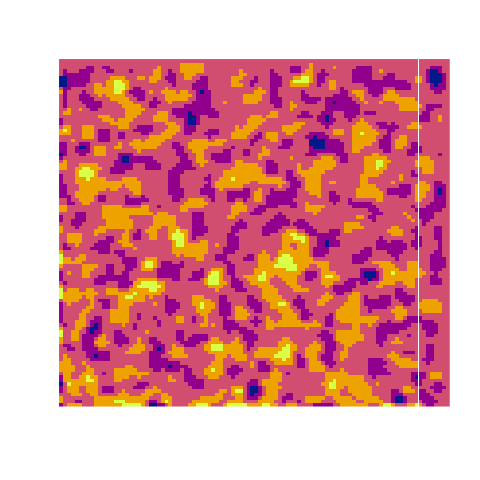
\includegraphics[width=\textwidth]{media/gauss_plasma.png}
        \caption{$C(|h|) = m \exp(-\frac{|h|^2}{a^2})$}
        \label{gauss plasma}
    \end{subfigure}
    \hfill
    \begin{subfigure}[b]{0.3\textwidth}
        \centering
        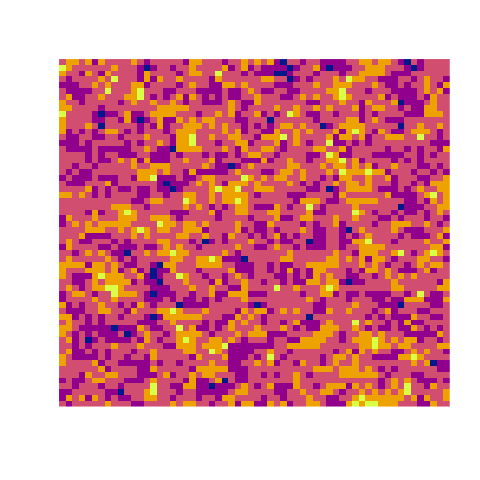
\includegraphics[width=\textwidth]{media/tent.png}
        \caption{$C(h) = \sigma^2(1 - \frac{|h|}{a})$}
        \label{fig:three sin x}
    \end{subfigure}
    \hfill
    \begin{subfigure}[b]{0.3\textwidth}
        \centering
        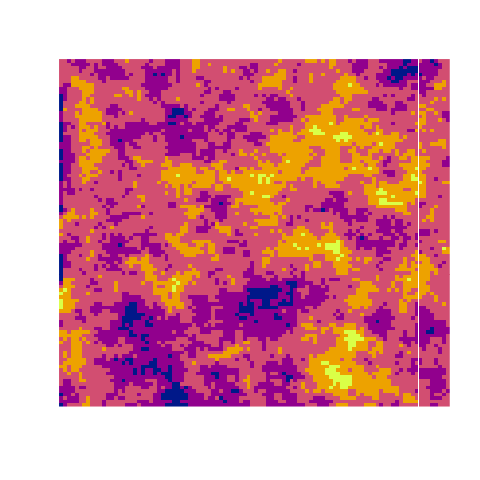
\includegraphics[width=\textwidth]{media/exp6_1.png}
        \caption{$C(h) = m \exp (-\frac{|h|}{a})$}
        \label{fig:five over x}
    \end{subfigure}
       \caption{En (a) on a une réalisation d'un champ gaussien avec fonction de covariance gaussienne. En (b) notre vecteur gaussien a pour modèle de covariance le modèle de tente.
       finalement en (c) on a un modèle exponentiel}
       \label{fig:three graphs}
\end{figure}

\newpage

\begin{figure}[h!]
    \centering
    \begin{subfigure}[b]{0.3\textwidth}
        \centering
        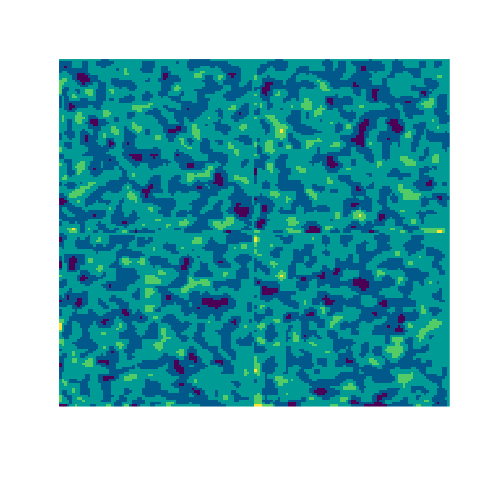
\includegraphics[width=\textwidth]{media/gauss_2.7_1_1.png}
        % \caption{$C(|h|) = m \exp(-\frac{|h|^2}{a^2})$}
        \label{gauss plasma}
    \end{subfigure}
    \hfill
    \begin{subfigure}[b]{0.3\textwidth}
        \centering
        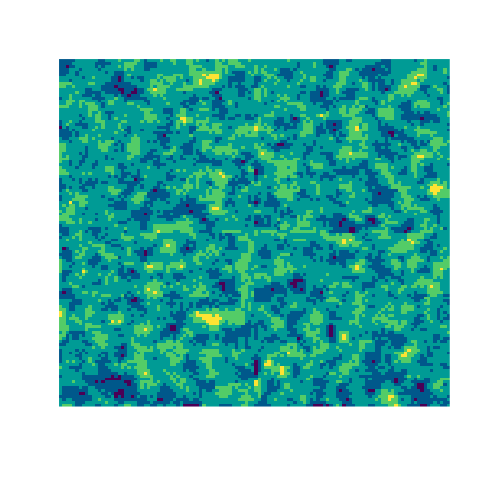
\includegraphics[width=\textwidth]{media/sphere.png}
        % \caption{Sphere}
        \label{fig:three sin x}
    \end{subfigure}
    \hfill
    \begin{subfigure}[b]{0.3\textwidth}
        \centering
        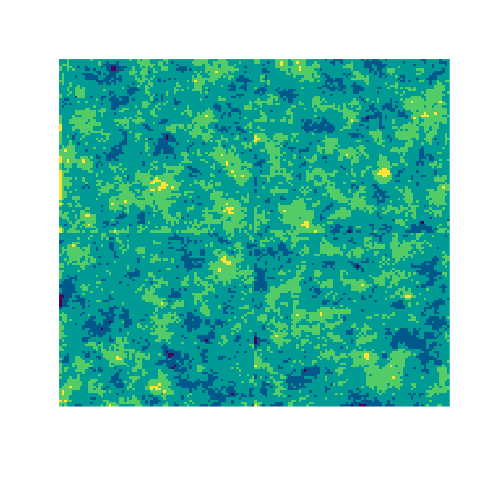
\includegraphics[width=\textwidth]{media/exp_2.png}
        % \caption{}
        \label{fig:five over x}
    \end{subfigure}
       \caption{Encore 3 réalisations d'un champ gaussien en quadrants. A gauche on a une covariance gaussienne, au milieu une covariance
       sphérique, et à droite une covariance exponentielle}
       \label{fig:three graphs}
\end{figure}

\subsubsection{Méthodologie}

%%Reprenons l'exemple d'une grille de $3$ lignes et $3$ colonnes. Pour simuler une réalisation de la fonction aléatoire $Z$, on procède en simulant
%%un vecteur gaussien de $9$ éléments, dont la matrice de covariance $\Sigma$ est déterminé par l'hypothèse de stationnarité forte (à l'ordre 1 et 2) et
%%calculé selon un modèle choisit. Nous utiliserons le modèle exponentielle pour commencer. Finalement, pour simplifier l'exemple on prend une espérance
%%$\mu = \textbf{0} \in \mathbb{R}^9$.

Prenons l'exemple d'une grille de $3$ lignes et $3$ colonnes. Pour simuler une réalisation de la fonction aléatoire $Z$ nous procédons à
la simulation d'un vecteur gaussien de $9$ éléments, dont la matrice de covariance $\Sigma$est déterminée par l'hypothèse de stationnarité
forte (aux ordres 1 et 2) et calculée selon un modèle choisi. Nous utiliserons le modèle exponentiel pour commencer. Enfin, pour simplifier
l'exemple, nous prenons une espérance $\mu = \textbf{0} \in \mathbb{R}^9$.

Pour simuler un vecteur gaussien dans $\mathbb{R}^9$, on a besoin d'une matrice de covariance de $9$ lignes et $9$ colonnes :
$$
\Sigma =
\begin{pmatrix}
    \mathrm{Cov}[s_1, s_1] & \dots & \mathrm{Cov}[s_1, s_9] \\
    \vdots & \ddots & \\
    \mathrm{Cov}[s_9, s_1] & \dots & \mathrm{Cov}[s_9, s_9]
\end{pmatrix}
$$

Sous l'hypothèse de stationnarité, pour $C(h)$ le modèle exponentiel et $d(s_i, s_j)$ la norme euclidienne des coordonnées
de $s_i$ et $s_j$, on réecrit :

$$
\Sigma =
\begin{pmatrix}
    C(d(s_1, s_1)) & \dots & C(d(s_1, s_9)) \\
    \vdots & \ddots & \\
    C(d(s_9, s_1)) & \dots & C(d(s_9, s_9))
\end{pmatrix}
$$

En calculant les distances, l'on a :
$$
\Sigma = C(H), \quad H =
\begin{pmatrix}
    0 & 1 & 2 & 1 & \sqrt{2} & \sqrt{5} & 2 & \sqrt{5} & 2\sqrt{2} \\
     & 0 & 1 & \sqrt{2} & 1 & \sqrt{2} & \sqrt{5} & 2 & \sqrt{5} \\
     &  & 0 & \sqrt{5} & \sqrt{2} & 1 & 2\sqrt{2} & \sqrt{5} & 2\\
     & & & 0 & 1 & 2 & 1 & \sqrt{2} & \sqrt{5} \\
     & & & & 0 & 1 & \sqrt{2} & 1 & \sqrt{2} \\
     & & & & & 0 & \sqrt{5} & \sqrt{2} & 1 \\
     & & & & & & 0 & 1 & 2 \\
     & & & & & & & 0 & 1 \\
     & & & & & & & & 0 \\
\end{pmatrix}
$$

%%Comme la matrice $\Sigma$ est symmétrique, on rempli que le partie triangulaire à droite de $H$ pour la rapidité. Illustrons l'un des calculs pour qu'on comprends
%%bien ce que l'on vient de calculer. Pour chaque ligne, on souhaiterait calculer la covariance entre une site fixe et \textbf{toutes} les autres sites.
%%Pour la première ligne, on a computé les distances entre $s_1$ et $s_i \in \{s_1, \dots, s_9\}$. Par exemple,

Comme la matrice $Sigma $ est symétrique, nous ne remplissons que la partie triangulaire supérieure de $H$ Illustrons
un des calculs pour bien comprendre ce que nous venons de calculer. Pour chaque ligne, nous souhaitons calculer la covariance
entre un site fixe et \textbf{tous} les autres sites. Pour la première ligne, nous avons calculé les distances entre
$s_1$ et $s_i \in \{s_1, \dots, s_9\}$.Par exemple,


\begin{align*}
    H_{1, 1} &= d(s_1, s_1) = ||(1, 1) - (1, 1)||_2 = 0 \\
    H_{1, 2} &= d(s_1, s_2) = ||(1, 1) - (1, 2)||_2 = 1 \\
    H_{1, 6} &= d(s_1, s_6) = ||(1, 1) - (2, 3)||_2 = \sqrt{5}.
\end{align*}

%%Une dernière étape c'est d'appliquer le modèle de covariance exponentielle $C(h; a) = \exp(\frac{-|h|}{a})$
%%pour tout élément $h$ de $H$ afin de trouver $\Sigma$, un comportement qui est implémenté par la fonction
%%\texttt{get\_cov\_matrix\_exp(n, a)} pour une grille de $n$ lignes et $n$ colonnes.
%%Pour notre exemple, on appelle \texttt{get\_cov\_matrix\_exp(3, 1)}.

Une dernière étape consiste à appliquer le modèle de covariance exponentielle $C(h ; a) = \exp(\frac{-|h|}{a})$ pour
tout élément $h$ de $H$ afin de trouver $\Sigma$, un comportement qui est mis en œuvre par la fonction \texttt{get\_cov\_matrix\_exp(n, a)}
pour une grille de $n$ lignes et $n$ colonnes. Dans notre exemple, nous appelons la fonction \texttt{get\_cov\_matrix\_exp(3, 1)}.


$$
\Sigma = C(H; 1) =
\begin{pmatrix}
    1.00 & 0.37 & 0.14 & 0.37 & 0.24 & 0.11 & 0.14 & 0.11 & 0.06 \\
    0.37 & 1.00 & 0.37 & 0.24 & 0.37 & 0.24 & 0.11 & 0.14 & 0.11 \\
    14 & 0.37 & 1.00 & 0.11 & 0.24 & 0.37 & 0.06 & 0.11 & 0.14 \\
    0.37 & 0.24 & 0.11 & 1.00 & 0.37 & 0.14 & 0.37 & 0.24 & 0.11 \\
    0.24 & 0.37 & 0.24 & 0.37 & 1.00 & 0.37 & 0.24 & 0.37 & 0.24 \\
    0.11 & 0.24 & 0.37 & 0.14 & 0.37 & 1.00 & 0.11 & 0.24 & 0.37 \\
    0.14 & 0.11 & 0.06 & 0.37 & 0.24 & 0.11 & 1.00 & 0.37 & 0.14 \\
    0.11 & 0.14 & 0.11 & 0.24 & 0.37 & 0.24 & 0.37 & 1.00 & 0.37 \\
    0.06 & 0.11 & 0.14 & 0.11 & 0.24 & 0.37 & 0.14 & 0.37 & 1.00 \\
\end{pmatrix}
$$

%%On pourrait appliquer des autres modèles de covariance pour changer la dépendance spatiale de notre fonction aléatoire:

Nous pourrions appliquer d'autres modèles de covariance pour modifier la dépendance spatiale de notre fonction aléatoire :

\begin{itemize}
    \item[] Modèle de tente :
    \[
        C(h; a, \sigma) = \left\{\begin{array}{lr}
            \sigma^2(1 - \frac{|h|}{a}), & \text{si } 0< |n|\leq a\\
            0 & \text{si } |h| > a
            \end{array}\right.
    \]

    \texttt{get\_cov\_matrix\_tent(3, 2, 1)}
    $$
    \Sigma = C(H; 2, 1) =
    \begin{pmatrix}
    1 & 0.50 & 0.00 & 0.50 & 0.29 & 0.00 & 0.00 & 0.00 & 0.00 \\
    0.50                       & 1.00 & 0.50 & 0.29 & 0.50 & 0.29 & 0.00 & 0.00 & 0.00 \\
    0.00                       & 0.50 & 1.00 & 0.00 & 0.29 & 0.50 & 0.00 & 0.00 & 0.00 \\
    0.50                       & 0.29 & 0.00 & 1.00 & 0.50 & 0.00 & 0.50 & 0.29 & 0.00 \\
    0.29                       & 0.50 & 0.29 & 0.50 & 1.00 & 0.50 & 0.29 & 0.50 & 0.29 \\
    0.00                       & 0.29 & 0.50 & 0.00 & 0.50 & 1.00 & 0.00 & 0.29 & 0.50 \\
    0.00                       & 0.00 & 0.00 & 0.50 & 0.29 & 0.00 & 1.00 & 0.50 & 0.00 \\
    0.00                       & 0.00 & 0.00 & 0.29 & 0.50 & 0.29 & 0.50 & 1.00 & 0.50 \\
    0.00                       & 0.00 & 0.00 & 0.00 & 0.29 & 0.50 & 0.00 & 0.50 & 1.00
    \end{pmatrix}
    $$

    Ainsi que le modèle sphérique
    \[
        C(|h|; a, m) = \left\{\begin{array}{lr}
            m(1 - (\frac{3}{2}\frac{|h|}{a} - \frac{1}{2}\frac{|h|^3}{a^3})), & \text{si } 0< |n|\leq a\\
            0 & \text{si } |h| > a
            \end{array}\right.
    \]et gaussien
    \[
        C(|h|; a, m) = \begin{array}{lr}
            m \exp (- \frac{|h|^2}{a^2}), & a > 0
            \end{array}
    \]
    restent à notre disposition avec nos implémentations \texttt{get\_cov\_matrix\_sphere} et
    \texttt{get\_cov\_matrix\_gauss}.

\end{itemize}

%%Maintenant on appelle notre fonction \texttt{rmvnorm} pour simuler un vecteur gaussien dans $\mathbb{R}^9$ avec espérance $0$ et
%%matrice de covariance $\Sigma = C(H; a)$ suivant un modèle exponentiel avec $a = 3$.

Nous appelons maintenant notre fonction \texttt{rmvnorm} pour simuler un vecteur gaussien dans $\mathbb{R}^9$ avec une espérance $0$ et
une matrice de covariance $\Sigma = C(H ; a)$ suivant un modèle exponentiel avec $a = 3$.

\newpage

\begin{figure}[h!]
    \centering
    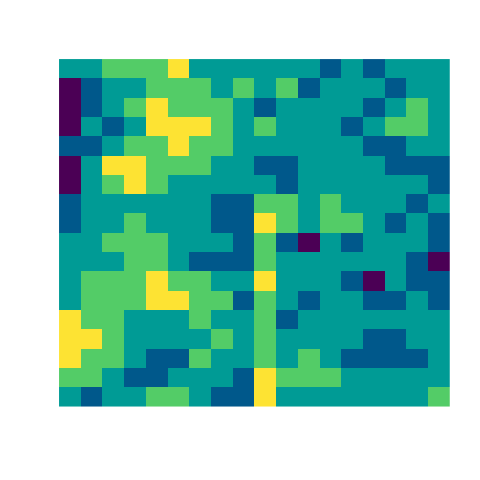
\includegraphics[width=5cm]{media/grid9.png}
    \caption{Réalisation $\omega \in \Omega$ d'un champ gaussien sur $\mathcal{D} \in \mathbb{R}^2$ dans $\mathbb{R}$ avec fonction de covariance exponentielle. Les valuers $Z(s)$ sont représenté en utilisant l'échelle
    de couleur \texttt{viridis}.}
\end{figure}

%%Pour élucider plus de structure, on fait augmenter la taille de notre grille. Cependant, comme la matrice de covariance est de taille $n^2$ lignes et $n^2$ colonnes pour une grille $n$ fois $n$, le nombre d'opérations juste pour
%%calculer $\Sigma$ est de complexité $\mathcal{O}(n^4)$! Et finalement la décomposition de Cholesky est de compléxité $\mathcal{O}(n^3)$ ainsi que la multiplication matricielle.

Pour élucider plus de structures, nous augmentons la taille de notre grille. Cependant, comme la matrice de covariance est de taille $n^2$
ligne et $n^2$ colonne pour une grille $n$ fois $n$ le nombre d'opérations droites pour calculer $\Sigma$ est de complexité $\mathcal{O}(n^4)$ .
Et enfin, la décomposition de Cholesky est de complexité $\mathcal{O}(n^3)$ ainsi que la multiplication de la matrice.

%%En résumé, cette méthode de simulation spatiale souffre de la malédiction des dimensions donc elle n'est pas traitable pour des grilles dont $n$
%%dépasse $100$. C'est ici où on pourrait parler des autre méthodes telle que la méthode spectrale pour simuler plus efficacement un champ gaussien de covariance
%%exponentielle.

En résumé, cette méthode de simulation spatiale souffre de la malédiction des dimensions et n'est donc pas exploitable pour des grilles
dont $n$ dépasse $100$. C'est là que nous pourrions parler d'autres méthodes comme la méthode spectrale pour simuler plus efficacement un
champ gaussien de covariance exponentielle.


\subsection{Krigeage} La dernière partie de notre projet s'oriente autour d'une méthode dite le krigéage, qui est effectivement une union de la simulation spatiale
avec le problème numérique des moindres carrés. Il s'agit d'un ensemble des observations $Z(s)$ pour un certain nombre de sites $s \in \mathcal{D}$. Par exemple, on pourrait
prendre $Z(s)$ la concentration d'une chimique sur la surface d'une région réctangulaire. Comme il est impossible d'observer la concentration à chaque site $s \in \mathbb{R}^2$,
on se contente d'observer un nombre fini de mesurements et en déduire les valeurs pour les autres sites dont la concentration est inconnue.

    Commencer avec un petit nombre de mesurements et en déduire le reste? Bien sûr qu'il s'agit d'un problème d'interpolation!

La formulation mathématique est la suivante : Donnée un ensemble de $n$ sites $\{s_1, \dots, s_n\}$ et leurs mesurements associés $Z(s_i)$, estimer
$\hat Z(s)$ pour tout $s \in \mathcal{D}$. La théorie c'est de construire un estimateur $\hat Z$ qui est exacte, c'est-à-dire que $\hat Z(s_i) = Z(s_i)$ pour
tout $s_i$ appartenant à l'ensemble des \textbf{observations}, et qui est formé d'une combinaison linéaire des observations connues :
$$ \hat Z(s) =  \sum \lambda_i Z(s_i).$$

Avec cette formulation, l'interpolation de krigeage se base sur la résolution d'un système linéaire dont
\begin{enumerate}
    \item Les poids $\lambda_i$ dépendent de $s$, le site que l'on souhaite estimer
    \item Le système à résoudre est gouverné pas la structure spatiale du modèle, la fonction de covariance $C(h)$.
\end{enumerate}

Avec cela en tête, on écrit le système à résoudre pour trouver les poids $\lambda_i$ au site $s$ que l'on voudrait estimer.
\begin{equation}
\begin{pmatrix}
    \text{Cov}[s_1, s_1] & \cdots & \text{Cov}[s_1, s_n] \\
    \vdots & \ddots & \vdots \\
    \text{Cov}[s_n, s_1] & \cdots & \text{Cov}[s_n, s_n] \\
\end{pmatrix}
\begin{pmatrix}
    \lambda_1 \\
    \vdots \\
    \lambda_n
\end{pmatrix}
=
\begin{pmatrix}
    \text{Cov}[s, s_1] \\
    \vdots \\
    \text{Cov}[s, s_n]
\end{pmatrix}
\end{equation}

Il est intéressant à remarquer que pour chaque $s \in \mathcal{D}$ dont on aimerait estimer $\hat Z(s)$, le système d'équations à résoudre de dépend
\textbf{pas} des valeurs observés $Z(s_i)$! Cela veut dire que l'importance de $Z(s_i)$ contribuant pour le calcul final $\hat Z(s_i)$, c'est-à-dire les poids $\lambda_i$, ne dépend \textbf{que}
sur la configuration spatiale des données. Le modèle de covariance utilisé détermine la valeur de chaque poids qui en revanche determinent la valeur de l'estimateur
$\hat Z(s)$. Sans tarder, étudierons un exemple avec $\mathcal{D} = \mathbb{R}^2$.

\subsubsection{Réalisation du krigeage}

Vu qu'on est pas munis des mesurements avec lesquelles on pourrait interpoler, on va utiliser la méthode décrite dans la dernière section pour simuler un champ gaussien
avec covariance exponentielle. Ensuite, on va échantilloner au hasard $n_{obs}$ sites et afin de réaliser l'interpolation spatiale. Commen\c cons avec une grille de 50 fois 50,
et nous prenons $n_{obs} = 100$.

Après la réalisation d'un champ gaussien, on va calculer $\hat Z(s)$ pour toute site dans notre grille, en résoulant un système d'équations \textbf{unique} pour chaque $s \in \mathcal{D}$, après
lequel on calcule la somme $$ \hat Z(s) =  \sum \lambda_i Z(s_i).$$


\begin{figure}[h!]
    \centering
    \begin{subfigure}[b]{0.3\textwidth}
        \centering
        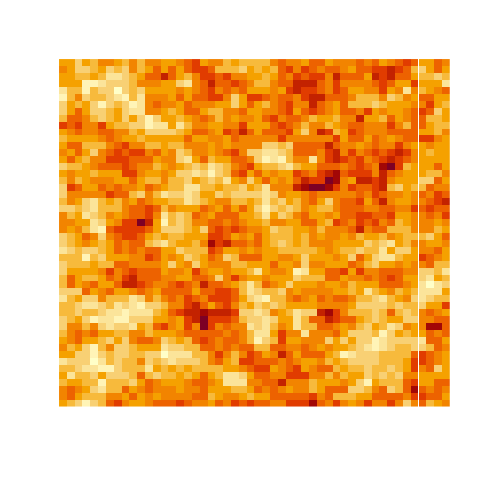
\includegraphics[width=\textwidth]{media/gauss_field_start.png}
        \caption{}
        \label{gauss plasma}
    \end{subfigure}
    \hfill
    \begin{subfigure}[b]{0.3\textwidth}
        \centering
        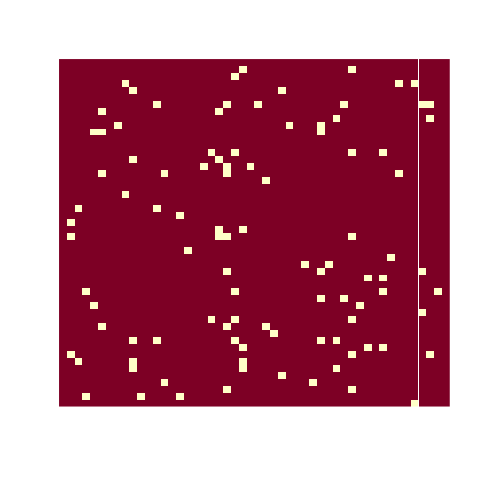
\includegraphics[width=\textwidth]{media/gauss_field_observations.png}
        \caption{}
        \label{fig:three sin x}
    \end{subfigure}
    \hfill
    \begin{subfigure}[b]{0.3\textwidth}
        \centering
        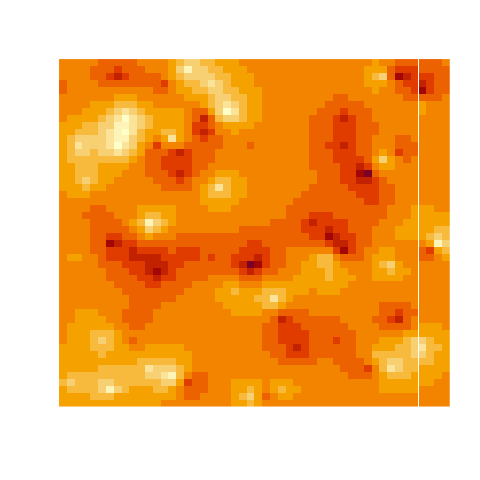
\includegraphics[width=\textwidth]{media/gauss_interp.png}
        \caption{}
        \label{fig:five over x}
    \end{subfigure}
       \caption{A gauche (a) on simule un champ gaussien avec une modèle de covariance exponentiel. En (b) on choisit aléatoirement 100 sites pour être nos
       observations. Pour (c) on résoud le problème de moindres carrés à \textbf{chaque site} pour calculer les $\lambda_i(s)$ utilisés dans le calcul final
       de l'estimateur $\hat Z$.}
       \label{fig:three graphs}
\end{figure}

Pour le plaisir on simule deux autres instances du krigeage

\begin{figure}[h!]
    \centering
    \begin{subfigure}[b]{0.3\textwidth}
        \centering
        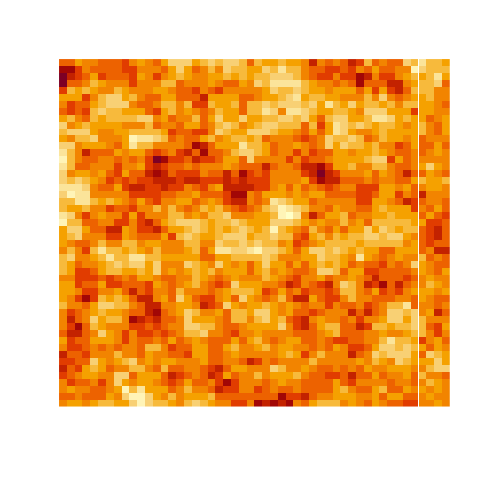
\includegraphics[width=\textwidth]{media/gauss_champ_1.png}
        % \caption{}
        \label{gauss plasma}
    \end{subfigure}
    \hfill
    \begin{subfigure}[b]{0.3\textwidth}
        \centering
        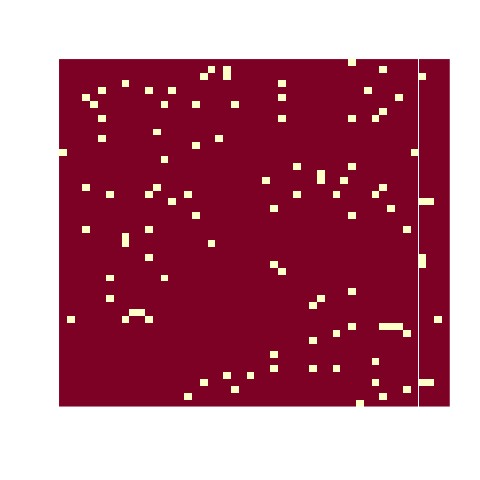
\includegraphics[width=\textwidth]{media/gauss_sites_1.png}
        % \caption{}
        \label{fig:three sin x}
    \end{subfigure}
    \hfill
    \begin{subfigure}[b]{0.3\textwidth}
        \centering
        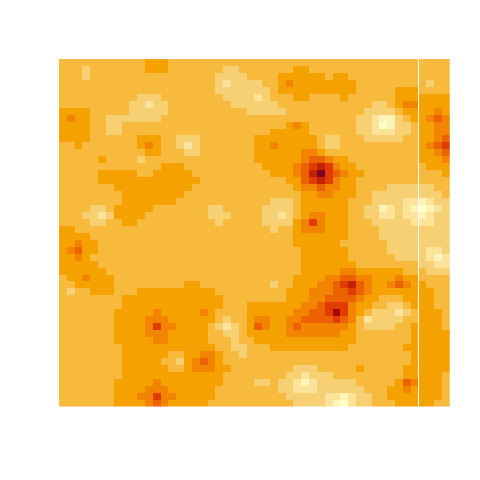
\includegraphics[width=\textwidth]{media/gauss_inter_1.png}
        % \caption{}
        \label{fig:five over x}
    \end{subfigure}
    %    \caption{A gauche (a) on simule un champ gaussien avec une modèle de covariance exponentiel. En (b) on choisit aléatoirement 100 sites pour être nos
    %    observations. Pour (c) on résoud le problème de moindres carrés à \textbf{chaque site} pour calculer les $\lambda_i(s)$ utilisés dans le calcul final
    %    de l'estimateur $\hat Z$.}
       \label{fig:three graphs}
\end{figure}
\vspace{-1.5cm}
\begin{figure}[h!]
    \centering
    \begin{subfigure}[b]{0.3\textwidth}
        \centering
        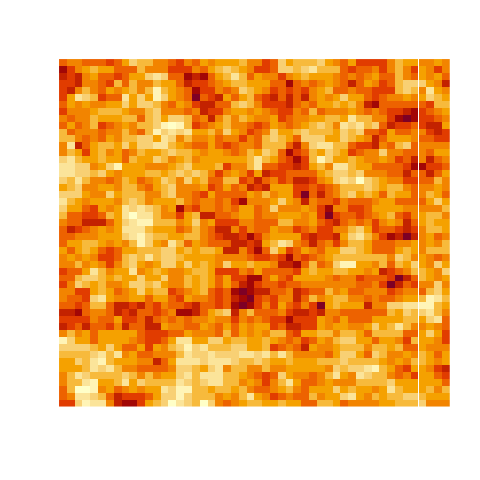
\includegraphics[width=\textwidth]{media/gauss_champ_2.png}
        % \caption{}
        \label{gauss plasma}
    \end{subfigure}
    \hfill
    \begin{subfigure}[b]{0.3\textwidth}
        \centering
        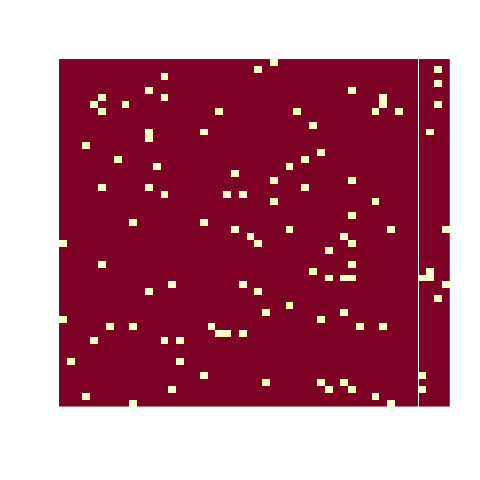
\includegraphics[width=\textwidth]{media/gauss_sites_2.png}
        % \caption{}
        \label{fig:three sin x}
    \end{subfigure}
    \hfill
    \begin{subfigure}[b]{0.3\textwidth}
        \centering
        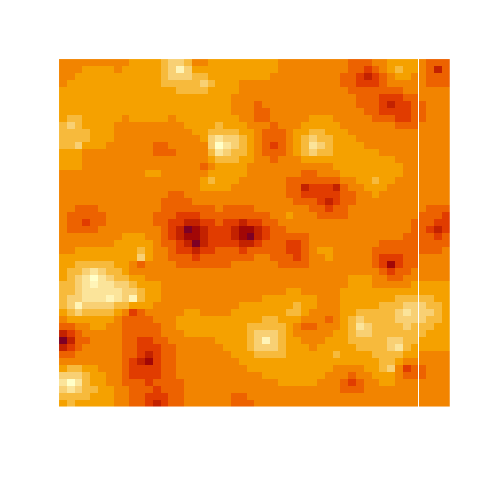
\includegraphics[width=\textwidth]{media/gauss_inter_2.png}
        % \caption{}
        \label{fig:five over x}
    \end{subfigure}
    %    \caption{A gauche (a) on simule un champ gaussien avec une modèle de covariance exponentiel. En (b) on choisit aléatoirement 100 sites pour être nos
    %    observations. Pour (c) on résoud le problème de moindres carrés à \textbf{chaque site} pour calculer les $\lambda_i(s)$ utilisés dans le calcul final
    %    de l'estimateur $\hat Z$.}
       \label{fig:three graphs}
\end{figure}

Ce qui est important à retenir c'est que les illustrations à droites ne sont pas censées à réproduire le champ à gauche avec lequel
on est partir. Ce qui fait le krigeage, comme l'interpolation polynômiale, c'est de toucher les bonnes valeurs où les mesurements ont été observés puis ensuite
estimer les valeurs inconnues entres les observations du sorte que l'espérance entre $\mathbb{E}[\hat Z(s) - Z(s)]$ soit minimisée. En appliquant cette stratégie envers
un ensemble des mesurements de profondeurs d'un câble sous-marin, on peut effectivement interpoler la profondeur entre les sites de mesurements afin de calculer sa longueur.

Malheuresement on a pas eu l'ocassion de travailler avec des données réelles, mais cela a été épanouissant d'aboutir la méthodologie spatiale.


\section{Programmation}
\subsection{R shiny}

Pour faire la simulation sans passer par du code R, nous avons créé une interface web afin de récupérer les variables simulées.
cette interface est implémentée avec la bibliothèque Rshiny, cette bibliothèque est simple à utiliser et permet de créer des sitewebs
avec des applications(fonctions) qui s'exécutent en arrière-plan pour faire la simulation.

Nous n'avons pas encore terminé de coder l'application mais dans la version finale l'utilisateur aura le choix de télécharger les variables
Aléatoires simulés.

\begin{figure}[h!]
    \centering
    \begin{subfigure}[b]{0.48\textwidth}
        \centering
        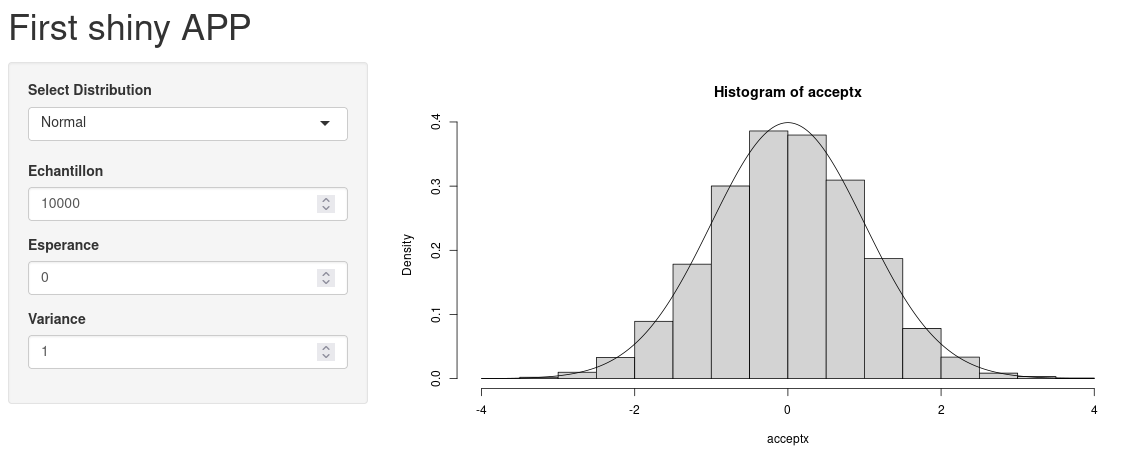
\includegraphics[width=\textwidth]{media/apppic1.png}
        % \caption{$C(|h|) = m \exp(-\frac{|h|^2}{a^2})$}
        \label{gauss plasma}
    \end{subfigure}
    \hfill
    \begin{subfigure}[b]{0.48\textwidth}
        \centering
        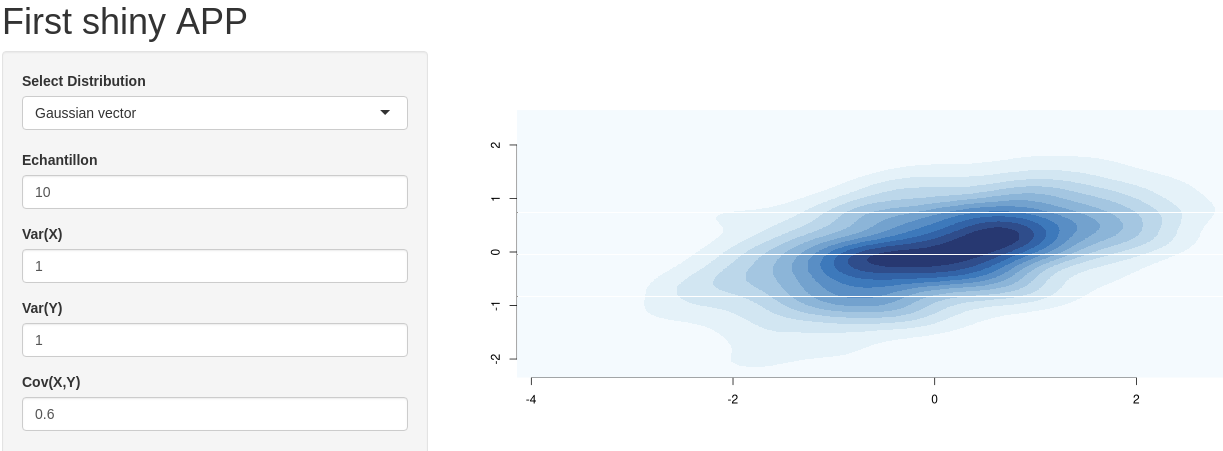
\includegraphics[width=\textwidth]{media/rshiny_gauss.png}
        % \caption{Sphere}
        \label{fig:three sin x}
    \end{subfigure}
    \caption{Captures d'écran de l'application shiny hébérgé \href{https://sousmarin.shinyapps.io/shinysousmarin/}{ici}}
\end{figure}

% \begin{figure}[h!]
% \centering
% 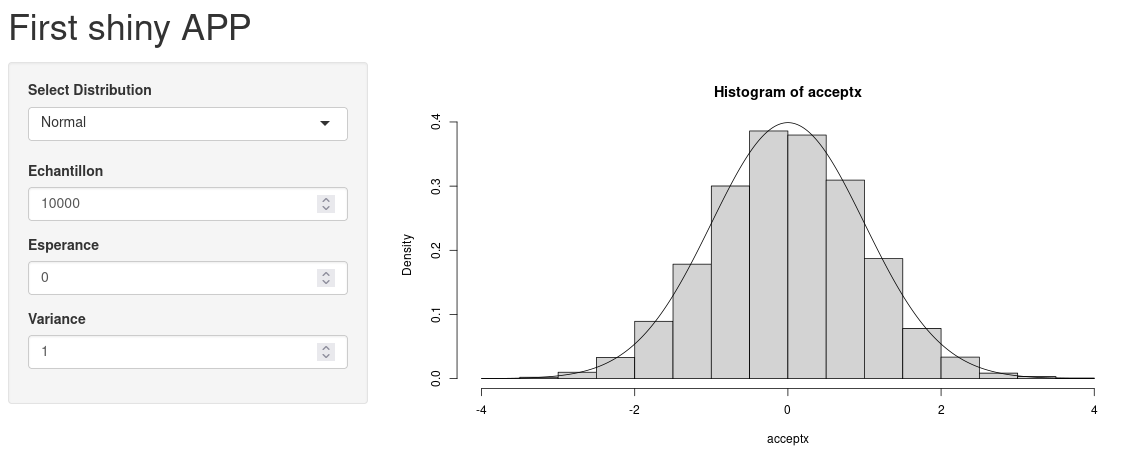
\includegraphics[width=\linewidth]{media/apppic1.png}
% \vspace{-5cm}
% \caption{1,000 réalisations d'une variable aléatoire normale avec espérance 0 et variance 1}
% \end{figure}

% \begin{figure}[h!]
% \centering
% 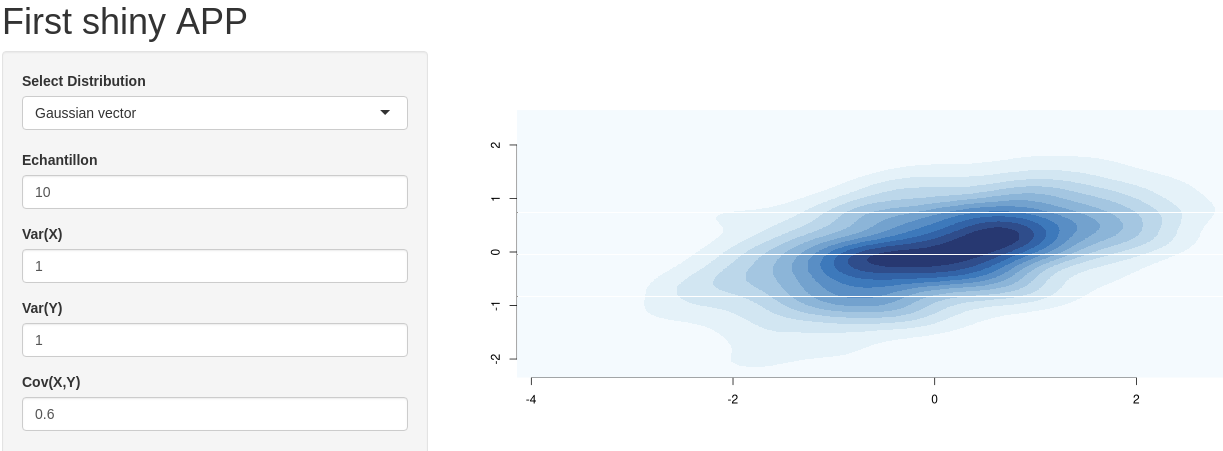
\includegraphics[width=\linewidth]{media/rshiny_gauss.png}
% \caption{Simulaton d'une loi gaussienne bivarié avec Cov$(X, Y) = 0.6$ et Var$(X)$ = Var$(Y) = 1$.}
% \end{figure}


\subsection{\texttt{sousmarin}}
Le package \texttt{R} \texttt{sousmarin} est disponible sur notre reperpertoire github \href{https://github.com/ejovo13/sousmarin}{ejovo13/sousmarin} avec les instructions pour comment télécharger la bibliothèque
sous \texttt{R} avec \texttt{install\_github} du package \texttt{devtools} écrit par le charmant Hadley Wickham.

Le package \texttt{sousmarin} contient les implémentations de toutes les méthodes que nous avons présentées dans ce rapport. La fonction d'acceptation-rejet pour une loi normale a été implémentée en \texttt{C++} en cohésion
avec le package \texttt{Rcpp} qui permet la compilation de code source en \texttt{C++} avec une interface en \texttt{R}. Aussi les fonctions pour générer la matrice de covariance pour une simulation
spatiale ont été réecrites en \texttt{C++} comme les boucles sont très lentes en \texttt{R}. Avant la réécriture, la fonction \texttt{get\_cov\_mat\_exp} mettait environ une minute pour simuler une grille
de dimension $60$ x $60$. Après l'implémentation en \texttt{C++} et nous avons réussi à effectuer une réalisation de $100$ x $100$ en moins de 10 secondes.

Toutes les fonctions utilisés pour les simulations font partie du package \texttt{sousmarin} et se trouve dans les répertoires \texttt{sousmarin/R} et \texttt{sousmarin/src}. Le code pour générer
les plots dans ce rapport se trouve sous le dossier \texttt{tex} du répo github.

\section{Conclusion}

Ainsi, nous avons commencé par simuler des variables aléatoires simples en se basant
uniquement sur runif (fonction uniforme de R). Nous savons maintenant utilisé les méthodes
 d'inversion et d'acceptation-rejet. Nous avons également poussé notre étude en simulation
 mutlivariée et en spatial. Pour cela nous avons utilisé les méthode  de krigeage et éventuellement
 nous allons voir si nous pouvons implémenter la méthode spectrale pour simuler des processus gaussiens

\section{Ce que nous pourrions amélirorer}
\subsection{Vitesse}

Les boucles en R sont péniblement lentes comparé aux autre languages compilés comme le C. Donc, la plupart de nos algorithmes implémentés sont
centaines des fois plus lentes que les fonctions de base en R telles que \texttt{runif}, \texttt{rexp}, etc. Si on avait plus de temps,
on aurait aimé implémenter les fonctions en C en utilisant le package Rcpp qui permet d'écrire notre propre code en C/C++ à executer sous R. Déjà on a pu implémenter
quelques fonctions problématiques en \texttt{C++} telles que calculer la matrice de covariance pour la simulation spatiale.

\subsection{Données}

On aurait aimé travaillé avec des données réelles afin de vraiment calculer la longuer d'un câble sous-marin. Cependant, on se contentait de
générer notre propre champ gaussien pour travailler la méthode de krigeage.

\subsection{Méthode spectrale}

La seule méthode de simulation qu'on avait visé mais que l'on a pas réussi à implémenter c'était la méthode spectrale.
Nommée spectrale pour ses liens avec l'analyse Fourier et sa méthodologie qui utilise des fonctions de base afin de simuler
un champ gaussien, cette méthode permet de simuler un vecteur gaussien d'un très grand dimension sans être frappé par la malédiction
de dimension.

\section{Réflexions}

\renewcommand {\epigraphflush} {flushleft}
\epigraph{Ce projet d'initiation a été une véritable découverte pour moi, puisque j'ai appris à
 utiliser de nouveaux langages de programmation, R et Rshiny. De plus, j'ai découvert la
  simulation de variables aléatoires multivariées qui sont utiles
lorsque l'on veut simuler certains phénomènes physiques.} {\textit{Samson}}

\epigraph{J'ai acquis de nombreuse compétence en informatique grâce à ce projet. J'ai appris à utiliser Github en projet,
le logiciel R et Rshiny. J'ai compris les notions d'aléatoire et pseudo-aléatoire.}
 {\textit{Pauline}}

\epigraph{J'ai approfindi mes connaissances autour la génération des variables aléatoires qui est indispensable dans le domaine
de processus stochastique ou des nombreuses phenomènes phsyiques sont modélisé par des fonctions aléatoires. J'ai eu ma première rencontre
avec la simulation conditionnelle et j'ai pu découvrir des nouveaux outils mathématiques utilisés en géostatistique tel que le variogram, la méthode spectrale,
et le krigeage.}
 {\textit{Evan}}


\newpage

\begin{thebibliography}{9}
    \bibitem{coursgeo}
    Yann Méneroux (2018), \emph{Introduction à la Géostatistique}, Institut National de l'Information Géographique et Forestièr
    \bibitem{texbook}
    Donald E. Knuth (1986) \emph{The \TeX{} Book}, Addison-Wesley Professional.

    \bibitem{acc rej}
    Karl Sigman (2007), \emph{Acceptance-Rejection Method}

    \bibitem{inv transform}
    Karl Sigman (2010), \emph{Inverse Transform Method}

    \bibitem{krig}
    Eric Marcon (2021), \emph{Krigeage avec R}

    \bibitem{handbook}
    Dikr P. Kroese (2011), Thomas Taimre, and Zdravko I. Botev, \emph{Handbook of Monte Carlo Methods}, Wiley series in Probability and Statistics

    \bibitem{variate generation}
    Luc Devroye (1986), \emph{Non-Uniform Random Variate Generation}, Springer Science

    \bibitem{geo sim}
    Christian Lantuéjoul (2002), \emph{Geostatistical Simulation}, Springer

    \bibitem{mont methods}
    Christian P. Robert, George Casella (1999), \emph{Monte Carlo Statistical Methods Second Edition}, Springer Texts in Statistics

    \bibitem{geostat}
    Jean-Paul Chilès, Pierre Delfiner (2012), \emph{Geostatistics Modeling Spatial Uncertainty}, Wiley series in Probability and Statistics

    \end{thebibliography}



\end{document}
